% Created by tikzDevice version 0.9 on 2016-03-14 23:38:47
% !TEX encoding = UTF-8 Unicode
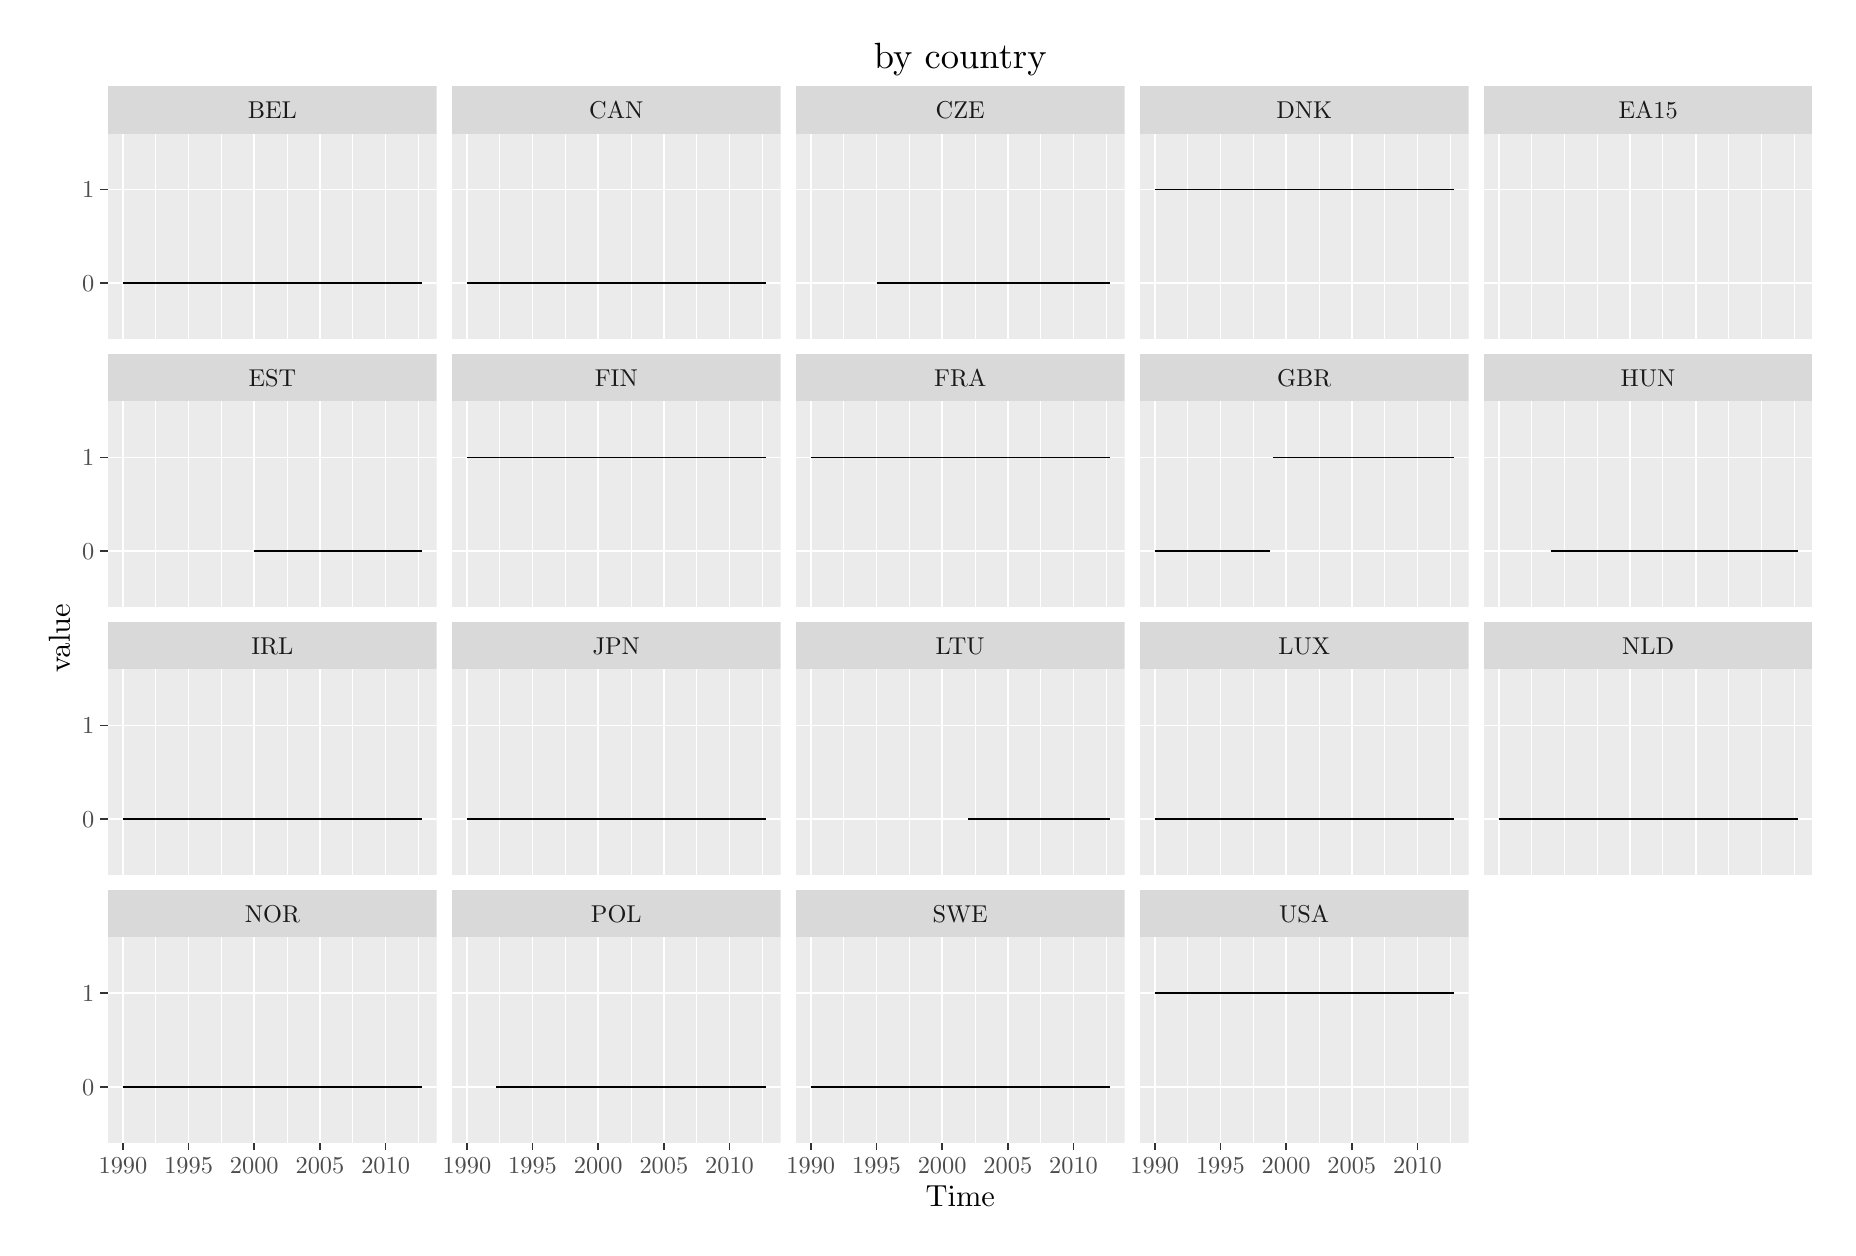
\begin{tikzpicture}[x=1pt,y=1pt]
\definecolor{fillColor}{RGB}{255,255,255}
\path[use as bounding box,fill=fillColor,fill opacity=0.00] (0,0) rectangle (650.43,433.62);
\begin{scope}
\path[clip] (  0.00,  0.00) rectangle (650.43,433.62);
\definecolor{drawColor}{RGB}{255,255,255}
\definecolor{fillColor}{RGB}{255,255,255}

\path[draw=drawColor,line width= 0.6pt,line join=round,line cap=round,fill=fillColor] (  0.00,  0.00) rectangle (650.43,433.62);
\end{scope}
\begin{scope}
\path[clip] ( 29.02,321.12) rectangle (147.81,395.37);
\definecolor{fillColor}{gray}{0.92}

\path[fill=fillColor] ( 29.02,321.12) rectangle (147.81,395.37);
\definecolor{drawColor}{RGB}{255,255,255}

\path[draw=drawColor,line width= 0.3pt,line join=round] ( 46.29,321.12) --
	( 46.29,395.37);

\path[draw=drawColor,line width= 0.3pt,line join=round] ( 70.02,321.12) --
	( 70.02,395.37);

\path[draw=drawColor,line width= 0.3pt,line join=round] ( 93.76,321.12) --
	( 93.76,395.37);

\path[draw=drawColor,line width= 0.3pt,line join=round] (117.49,321.12) --
	(117.49,395.37);

\path[draw=drawColor,line width= 0.3pt,line join=round] (141.22,321.12) --
	(141.22,395.37);

\path[draw=drawColor,line width= 0.6pt,line join=round] ( 29.02,341.37) --
	(147.81,341.37);

\path[draw=drawColor,line width= 0.6pt,line join=round] ( 29.02,375.12) --
	(147.81,375.12);

\path[draw=drawColor,line width= 0.6pt,line join=round] ( 34.42,321.12) --
	( 34.42,395.37);

\path[draw=drawColor,line width= 0.6pt,line join=round] ( 58.16,321.12) --
	( 58.16,395.37);

\path[draw=drawColor,line width= 0.6pt,line join=round] ( 81.89,321.12) --
	( 81.89,395.37);

\path[draw=drawColor,line width= 0.6pt,line join=round] (105.62,321.12) --
	(105.62,395.37);

\path[draw=drawColor,line width= 0.6pt,line join=round] (129.35,321.12) --
	(129.35,395.37);
\definecolor{drawColor}{RGB}{0,0,0}

\path[draw=drawColor,line width= 0.6pt,line join=round] ( 34.42,341.37) --
	( 35.61,341.37) --
	( 36.80,341.37) --
	( 37.98,341.37) --
	( 39.17,341.37) --
	( 40.36,341.37) --
	( 41.54,341.37) --
	( 42.73,341.37) --
	( 43.92,341.37) --
	( 45.10,341.37) --
	( 46.29,341.37) --
	( 47.48,341.37) --
	( 48.66,341.37) --
	( 49.85,341.37) --
	( 51.04,341.37) --
	( 52.22,341.37) --
	( 53.41,341.37) --
	( 54.60,341.37) --
	( 55.78,341.37) --
	( 56.97,341.37) --
	( 58.16,341.37) --
	( 59.34,341.37) --
	( 60.53,341.37) --
	( 61.72,341.37) --
	( 62.90,341.37) --
	( 64.09,341.37) --
	( 65.28,341.37) --
	( 66.46,341.37) --
	( 67.65,341.37) --
	( 68.84,341.37) --
	( 70.02,341.37) --
	( 71.21,341.37) --
	( 72.40,341.37) --
	( 73.58,341.37) --
	( 74.77,341.37) --
	( 75.96,341.37) --
	( 77.14,341.37) --
	( 78.33,341.37) --
	( 79.52,341.37) --
	( 80.70,341.37) --
	( 81.89,341.37) --
	( 83.08,341.37) --
	( 84.26,341.37) --
	( 85.45,341.37) --
	( 86.64,341.37) --
	( 87.82,341.37) --
	( 89.01,341.37) --
	( 90.20,341.37) --
	( 91.38,341.37) --
	( 92.57,341.37) --
	( 93.76,341.37) --
	( 94.94,341.37) --
	( 96.13,341.37) --
	( 97.32,341.37) --
	( 98.50,341.37) --
	( 99.69,341.37) --
	(100.87,341.37) --
	(102.06,341.37) --
	(103.25,341.37) --
	(104.43,341.37) --
	(105.62,341.37) --
	(106.81,341.37) --
	(107.99,341.37) --
	(109.18,341.37) --
	(110.37,341.37) --
	(111.55,341.37) --
	(112.74,341.37) --
	(113.93,341.37) --
	(115.11,341.37) --
	(116.30,341.37) --
	(117.49,341.37) --
	(118.67,341.37) --
	(119.86,341.37) --
	(121.05,341.37) --
	(122.23,341.37) --
	(123.42,341.37) --
	(124.61,341.37) --
	(125.79,341.37) --
	(126.98,341.37) --
	(128.17,341.37) --
	(129.35,341.37) --
	(130.54,341.37) --
	(131.73,341.37) --
	(132.91,341.37) --
	(134.10,341.37) --
	(135.29,341.37) --
	(136.47,341.37) --
	(137.66,341.37) --
	(138.85,341.37) --
	(140.03,341.37) --
	(141.22,341.37) --
	(142.41,341.37);
\end{scope}
\begin{scope}
\path[clip] (153.31,321.12) rectangle (272.09,395.37);
\definecolor{fillColor}{gray}{0.92}

\path[fill=fillColor] (153.31,321.12) rectangle (272.09,395.37);
\definecolor{drawColor}{RGB}{255,255,255}

\path[draw=drawColor,line width= 0.3pt,line join=round] (170.57,321.12) --
	(170.57,395.37);

\path[draw=drawColor,line width= 0.3pt,line join=round] (194.30,321.12) --
	(194.30,395.37);

\path[draw=drawColor,line width= 0.3pt,line join=round] (218.04,321.12) --
	(218.04,395.37);

\path[draw=drawColor,line width= 0.3pt,line join=round] (241.77,321.12) --
	(241.77,395.37);

\path[draw=drawColor,line width= 0.3pt,line join=round] (265.50,321.12) --
	(265.50,395.37);

\path[draw=drawColor,line width= 0.6pt,line join=round] (153.31,341.37) --
	(272.09,341.37);

\path[draw=drawColor,line width= 0.6pt,line join=round] (153.31,375.12) --
	(272.09,375.12);

\path[draw=drawColor,line width= 0.6pt,line join=round] (158.71,321.12) --
	(158.71,395.37);

\path[draw=drawColor,line width= 0.6pt,line join=round] (182.44,321.12) --
	(182.44,395.37);

\path[draw=drawColor,line width= 0.6pt,line join=round] (206.17,321.12) --
	(206.17,395.37);

\path[draw=drawColor,line width= 0.6pt,line join=round] (229.90,321.12) --
	(229.90,395.37);

\path[draw=drawColor,line width= 0.6pt,line join=round] (253.63,321.12) --
	(253.63,395.37);
\definecolor{drawColor}{RGB}{0,0,0}

\path[draw=drawColor,line width= 0.6pt,line join=round] (158.71,341.37) --
	(159.89,341.37) --
	(161.08,341.37) --
	(162.26,341.37) --
	(163.45,341.37) --
	(164.64,341.37) --
	(165.82,341.37) --
	(167.01,341.37) --
	(168.20,341.37) --
	(169.38,341.37) --
	(170.57,341.37) --
	(171.76,341.37) --
	(172.94,341.37) --
	(174.13,341.37) --
	(175.32,341.37) --
	(176.50,341.37) --
	(177.69,341.37) --
	(178.88,341.37) --
	(180.06,341.37) --
	(181.25,341.37) --
	(182.44,341.37) --
	(183.62,341.37) --
	(184.81,341.37) --
	(186.00,341.37) --
	(187.18,341.37) --
	(188.37,341.37) --
	(189.56,341.37) --
	(190.74,341.37) --
	(191.93,341.37) --
	(193.12,341.37) --
	(194.30,341.37) --
	(195.49,341.37) --
	(196.68,341.37) --
	(197.86,341.37) --
	(199.05,341.37) --
	(200.24,341.37) --
	(201.42,341.37) --
	(202.61,341.37) --
	(203.80,341.37) --
	(204.98,341.37) --
	(206.17,341.37) --
	(207.36,341.37) --
	(208.54,341.37) --
	(209.73,341.37) --
	(210.92,341.37) --
	(212.10,341.37) --
	(213.29,341.37) --
	(214.48,341.37) --
	(215.66,341.37) --
	(216.85,341.37) --
	(218.04,341.37) --
	(219.22,341.37) --
	(220.41,341.37) --
	(221.60,341.37) --
	(222.78,341.37) --
	(223.97,341.37) --
	(225.16,341.37) --
	(226.34,341.37) --
	(227.53,341.37) --
	(228.72,341.37) --
	(229.90,341.37) --
	(231.09,341.37) --
	(232.28,341.37) --
	(233.46,341.37) --
	(234.65,341.37) --
	(235.84,341.37) --
	(237.02,341.37) --
	(238.21,341.37) --
	(239.40,341.37) --
	(240.58,341.37) --
	(241.77,341.37) --
	(242.96,341.37) --
	(244.14,341.37) --
	(245.33,341.37) --
	(246.52,341.37) --
	(247.70,341.37) --
	(248.89,341.37) --
	(250.08,341.37) --
	(251.26,341.37) --
	(252.45,341.37) --
	(253.63,341.37) --
	(254.82,341.37) --
	(256.01,341.37) --
	(257.19,341.37) --
	(258.38,341.37) --
	(259.57,341.37) --
	(260.75,341.37) --
	(261.94,341.37) --
	(263.13,341.37) --
	(264.31,341.37) --
	(265.50,341.37) --
	(266.69,341.37);
\end{scope}
\begin{scope}
\path[clip] (277.59,321.12) rectangle (396.37,395.37);
\definecolor{fillColor}{gray}{0.92}

\path[fill=fillColor] (277.59,321.12) rectangle (396.37,395.37);
\definecolor{drawColor}{RGB}{255,255,255}

\path[draw=drawColor,line width= 0.3pt,line join=round] (294.85,321.12) --
	(294.85,395.37);

\path[draw=drawColor,line width= 0.3pt,line join=round] (318.58,321.12) --
	(318.58,395.37);

\path[draw=drawColor,line width= 0.3pt,line join=round] (342.32,321.12) --
	(342.32,395.37);

\path[draw=drawColor,line width= 0.3pt,line join=round] (366.05,321.12) --
	(366.05,395.37);

\path[draw=drawColor,line width= 0.3pt,line join=round] (389.78,321.12) --
	(389.78,395.37);

\path[draw=drawColor,line width= 0.6pt,line join=round] (277.59,341.37) --
	(396.37,341.37);

\path[draw=drawColor,line width= 0.6pt,line join=round] (277.59,375.12) --
	(396.37,375.12);

\path[draw=drawColor,line width= 0.6pt,line join=round] (282.99,321.12) --
	(282.99,395.37);

\path[draw=drawColor,line width= 0.6pt,line join=round] (306.72,321.12) --
	(306.72,395.37);

\path[draw=drawColor,line width= 0.6pt,line join=round] (330.45,321.12) --
	(330.45,395.37);

\path[draw=drawColor,line width= 0.6pt,line join=round] (354.18,321.12) --
	(354.18,395.37);

\path[draw=drawColor,line width= 0.6pt,line join=round] (377.92,321.12) --
	(377.92,395.37);
\definecolor{drawColor}{RGB}{0,0,0}

\path[draw=drawColor,line width= 0.6pt,line join=round] (306.72,341.37) --
	(307.91,341.37) --
	(309.09,341.37) --
	(310.28,341.37) --
	(311.47,341.37) --
	(312.65,341.37) --
	(313.84,341.37) --
	(315.02,341.37) --
	(316.21,341.37) --
	(317.40,341.37) --
	(318.58,341.37) --
	(319.77,341.37) --
	(320.96,341.37) --
	(322.14,341.37) --
	(323.33,341.37) --
	(324.52,341.37) --
	(325.70,341.37) --
	(326.89,341.37) --
	(328.08,341.37) --
	(329.26,341.37) --
	(330.45,341.37) --
	(331.64,341.37) --
	(332.82,341.37) --
	(334.01,341.37) --
	(335.20,341.37) --
	(336.38,341.37) --
	(337.57,341.37) --
	(338.76,341.37) --
	(339.94,341.37) --
	(341.13,341.37) --
	(342.32,341.37) --
	(343.50,341.37) --
	(344.69,341.37) --
	(345.88,341.37) --
	(347.06,341.37) --
	(348.25,341.37) --
	(349.44,341.37) --
	(350.62,341.37) --
	(351.81,341.37) --
	(353.00,341.37) --
	(354.18,341.37) --
	(355.37,341.37) --
	(356.56,341.37) --
	(357.74,341.37) --
	(358.93,341.37) --
	(360.12,341.37) --
	(361.30,341.37) --
	(362.49,341.37) --
	(363.68,341.37) --
	(364.86,341.37) --
	(366.05,341.37) --
	(367.24,341.37) --
	(368.42,341.37) --
	(369.61,341.37) --
	(370.80,341.37) --
	(371.98,341.37) --
	(373.17,341.37) --
	(374.36,341.37) --
	(375.54,341.37) --
	(376.73,341.37) --
	(377.92,341.37) --
	(379.10,341.37) --
	(380.29,341.37) --
	(381.48,341.37) --
	(382.66,341.37) --
	(383.85,341.37) --
	(385.04,341.37) --
	(386.22,341.37) --
	(387.41,341.37) --
	(388.60,341.37) --
	(389.78,341.37) --
	(390.97,341.37);
\end{scope}
\begin{scope}
\path[clip] (401.87,321.12) rectangle (520.65,395.37);
\definecolor{fillColor}{gray}{0.92}

\path[fill=fillColor] (401.87,321.12) rectangle (520.65,395.37);
\definecolor{drawColor}{RGB}{255,255,255}

\path[draw=drawColor,line width= 0.3pt,line join=round] (419.13,321.12) --
	(419.13,395.37);

\path[draw=drawColor,line width= 0.3pt,line join=round] (442.87,321.12) --
	(442.87,395.37);

\path[draw=drawColor,line width= 0.3pt,line join=round] (466.60,321.12) --
	(466.60,395.37);

\path[draw=drawColor,line width= 0.3pt,line join=round] (490.33,321.12) --
	(490.33,395.37);

\path[draw=drawColor,line width= 0.3pt,line join=round] (514.06,321.12) --
	(514.06,395.37);

\path[draw=drawColor,line width= 0.6pt,line join=round] (401.87,341.37) --
	(520.65,341.37);

\path[draw=drawColor,line width= 0.6pt,line join=round] (401.87,375.12) --
	(520.65,375.12);

\path[draw=drawColor,line width= 0.6pt,line join=round] (407.27,321.12) --
	(407.27,395.37);

\path[draw=drawColor,line width= 0.6pt,line join=round] (431.00,321.12) --
	(431.00,395.37);

\path[draw=drawColor,line width= 0.6pt,line join=round] (454.73,321.12) --
	(454.73,395.37);

\path[draw=drawColor,line width= 0.6pt,line join=round] (478.46,321.12) --
	(478.46,395.37);

\path[draw=drawColor,line width= 0.6pt,line join=round] (502.20,321.12) --
	(502.20,395.37);
\definecolor{drawColor}{RGB}{0,0,0}

\path[draw=drawColor,line width= 0.6pt,line join=round] (407.27,375.12) --
	(408.45,375.12) --
	(409.64,375.12) --
	(410.83,375.12) --
	(412.01,375.12) --
	(413.20,375.12) --
	(414.39,375.12) --
	(415.57,375.12) --
	(416.76,375.12) --
	(417.95,375.12) --
	(419.13,375.12) --
	(420.32,375.12) --
	(421.51,375.12) --
	(422.69,375.12) --
	(423.88,375.12) --
	(425.07,375.12) --
	(426.25,375.12) --
	(427.44,375.12) --
	(428.63,375.12) --
	(429.81,375.12) --
	(431.00,375.12) --
	(432.19,375.12) --
	(433.37,375.12) --
	(434.56,375.12) --
	(435.75,375.12) --
	(436.93,375.12) --
	(438.12,375.12) --
	(439.31,375.12) --
	(440.49,375.12) --
	(441.68,375.12) --
	(442.87,375.12) --
	(444.05,375.12) --
	(445.24,375.12) --
	(446.43,375.12) --
	(447.61,375.12) --
	(448.80,375.12) --
	(449.99,375.12) --
	(451.17,375.12) --
	(452.36,375.12) --
	(453.55,375.12) --
	(454.73,375.12) --
	(455.92,375.12) --
	(457.11,375.12) --
	(458.29,375.12) --
	(459.48,375.12) --
	(460.67,375.12) --
	(461.85,375.12) --
	(463.04,375.12) --
	(464.23,375.12) --
	(465.41,375.12) --
	(466.60,375.12) --
	(467.78,375.12) --
	(468.97,375.12) --
	(470.16,375.12) --
	(471.34,375.12) --
	(472.53,375.12) --
	(473.72,375.12) --
	(474.90,375.12) --
	(476.09,375.12) --
	(477.28,375.12) --
	(478.46,375.12) --
	(479.65,375.12) --
	(480.84,375.12) --
	(482.02,375.12) --
	(483.21,375.12) --
	(484.40,375.12) --
	(485.58,375.12) --
	(486.77,375.12) --
	(487.96,375.12) --
	(489.14,375.12) --
	(490.33,375.12) --
	(491.52,375.12) --
	(492.70,375.12) --
	(493.89,375.12) --
	(495.08,375.12) --
	(496.26,375.12) --
	(497.45,375.12) --
	(498.64,375.12) --
	(499.82,375.12) --
	(501.01,375.12) --
	(502.20,375.12) --
	(503.38,375.12) --
	(504.57,375.12) --
	(505.76,375.12) --
	(506.94,375.12) --
	(508.13,375.12) --
	(509.32,375.12) --
	(510.50,375.12) --
	(511.69,375.12) --
	(512.88,375.12) --
	(514.06,375.12) --
	(515.25,375.12);
\end{scope}
\begin{scope}
\path[clip] (526.15,321.12) rectangle (644.93,395.37);
\definecolor{fillColor}{gray}{0.92}

\path[fill=fillColor] (526.15,321.12) rectangle (644.93,395.37);
\definecolor{drawColor}{RGB}{255,255,255}

\path[draw=drawColor,line width= 0.3pt,line join=round] (543.41,321.12) --
	(543.41,395.37);

\path[draw=drawColor,line width= 0.3pt,line join=round] (567.15,321.12) --
	(567.15,395.37);

\path[draw=drawColor,line width= 0.3pt,line join=round] (590.88,321.12) --
	(590.88,395.37);

\path[draw=drawColor,line width= 0.3pt,line join=round] (614.61,321.12) --
	(614.61,395.37);

\path[draw=drawColor,line width= 0.3pt,line join=round] (638.34,321.12) --
	(638.34,395.37);

\path[draw=drawColor,line width= 0.6pt,line join=round] (526.15,341.37) --
	(644.93,341.37);

\path[draw=drawColor,line width= 0.6pt,line join=round] (526.15,375.12) --
	(644.93,375.12);

\path[draw=drawColor,line width= 0.6pt,line join=round] (531.55,321.12) --
	(531.55,395.37);

\path[draw=drawColor,line width= 0.6pt,line join=round] (555.28,321.12) --
	(555.28,395.37);

\path[draw=drawColor,line width= 0.6pt,line join=round] (579.01,321.12) --
	(579.01,395.37);

\path[draw=drawColor,line width= 0.6pt,line join=round] (602.75,321.12) --
	(602.75,395.37);

\path[draw=drawColor,line width= 0.6pt,line join=round] (626.48,321.12) --
	(626.48,395.37);
\end{scope}
\begin{scope}
\path[clip] ( 29.02,224.31) rectangle (147.81,298.56);
\definecolor{fillColor}{gray}{0.92}

\path[fill=fillColor] ( 29.02,224.31) rectangle (147.81,298.56);
\definecolor{drawColor}{RGB}{255,255,255}

\path[draw=drawColor,line width= 0.3pt,line join=round] ( 46.29,224.31) --
	( 46.29,298.56);

\path[draw=drawColor,line width= 0.3pt,line join=round] ( 70.02,224.31) --
	( 70.02,298.56);

\path[draw=drawColor,line width= 0.3pt,line join=round] ( 93.76,224.31) --
	( 93.76,298.56);

\path[draw=drawColor,line width= 0.3pt,line join=round] (117.49,224.31) --
	(117.49,298.56);

\path[draw=drawColor,line width= 0.3pt,line join=round] (141.22,224.31) --
	(141.22,298.56);

\path[draw=drawColor,line width= 0.6pt,line join=round] ( 29.02,244.56) --
	(147.81,244.56);

\path[draw=drawColor,line width= 0.6pt,line join=round] ( 29.02,278.31) --
	(147.81,278.31);

\path[draw=drawColor,line width= 0.6pt,line join=round] ( 34.42,224.31) --
	( 34.42,298.56);

\path[draw=drawColor,line width= 0.6pt,line join=round] ( 58.16,224.31) --
	( 58.16,298.56);

\path[draw=drawColor,line width= 0.6pt,line join=round] ( 81.89,224.31) --
	( 81.89,298.56);

\path[draw=drawColor,line width= 0.6pt,line join=round] (105.62,224.31) --
	(105.62,298.56);

\path[draw=drawColor,line width= 0.6pt,line join=round] (129.35,224.31) --
	(129.35,298.56);
\definecolor{drawColor}{RGB}{0,0,0}

\path[draw=drawColor,line width= 0.6pt,line join=round] ( 81.89,244.56) --
	( 83.08,244.56) --
	( 84.26,244.56) --
	( 85.45,244.56) --
	( 86.64,244.56) --
	( 87.82,244.56) --
	( 89.01,244.56) --
	( 90.20,244.56) --
	( 91.38,244.56) --
	( 92.57,244.56) --
	( 93.76,244.56) --
	( 94.94,244.56) --
	( 96.13,244.56) --
	( 97.32,244.56) --
	( 98.50,244.56) --
	( 99.69,244.56) --
	(100.87,244.56) --
	(102.06,244.56) --
	(103.25,244.56) --
	(104.43,244.56) --
	(105.62,244.56) --
	(106.81,244.56) --
	(107.99,244.56) --
	(109.18,244.56) --
	(110.37,244.56) --
	(111.55,244.56) --
	(112.74,244.56) --
	(113.93,244.56) --
	(115.11,244.56) --
	(116.30,244.56) --
	(117.49,244.56) --
	(118.67,244.56) --
	(119.86,244.56) --
	(121.05,244.56) --
	(122.23,244.56) --
	(123.42,244.56) --
	(124.61,244.56) --
	(125.79,244.56) --
	(126.98,244.56) --
	(128.17,244.56) --
	(129.35,244.56) --
	(130.54,244.56) --
	(131.73,244.56) --
	(132.91,244.56) --
	(134.10,244.56) --
	(135.29,244.56) --
	(136.47,244.56) --
	(137.66,244.56) --
	(138.85,244.56) --
	(140.03,244.56) --
	(141.22,244.56) --
	(142.41,244.56);
\end{scope}
\begin{scope}
\path[clip] (153.31,224.31) rectangle (272.09,298.56);
\definecolor{fillColor}{gray}{0.92}

\path[fill=fillColor] (153.31,224.31) rectangle (272.09,298.56);
\definecolor{drawColor}{RGB}{255,255,255}

\path[draw=drawColor,line width= 0.3pt,line join=round] (170.57,224.31) --
	(170.57,298.56);

\path[draw=drawColor,line width= 0.3pt,line join=round] (194.30,224.31) --
	(194.30,298.56);

\path[draw=drawColor,line width= 0.3pt,line join=round] (218.04,224.31) --
	(218.04,298.56);

\path[draw=drawColor,line width= 0.3pt,line join=round] (241.77,224.31) --
	(241.77,298.56);

\path[draw=drawColor,line width= 0.3pt,line join=round] (265.50,224.31) --
	(265.50,298.56);

\path[draw=drawColor,line width= 0.6pt,line join=round] (153.31,244.56) --
	(272.09,244.56);

\path[draw=drawColor,line width= 0.6pt,line join=round] (153.31,278.31) --
	(272.09,278.31);

\path[draw=drawColor,line width= 0.6pt,line join=round] (158.71,224.31) --
	(158.71,298.56);

\path[draw=drawColor,line width= 0.6pt,line join=round] (182.44,224.31) --
	(182.44,298.56);

\path[draw=drawColor,line width= 0.6pt,line join=round] (206.17,224.31) --
	(206.17,298.56);

\path[draw=drawColor,line width= 0.6pt,line join=round] (229.90,224.31) --
	(229.90,298.56);

\path[draw=drawColor,line width= 0.6pt,line join=round] (253.63,224.31) --
	(253.63,298.56);
\definecolor{drawColor}{RGB}{0,0,0}

\path[draw=drawColor,line width= 0.6pt,line join=round] (158.71,278.31) --
	(159.89,278.31) --
	(161.08,278.31) --
	(162.26,278.31) --
	(163.45,278.31) --
	(164.64,278.31) --
	(165.82,278.31) --
	(167.01,278.31) --
	(168.20,278.31) --
	(169.38,278.31) --
	(170.57,278.31) --
	(171.76,278.31) --
	(172.94,278.31) --
	(174.13,278.31) --
	(175.32,278.31) --
	(176.50,278.31) --
	(177.69,278.31) --
	(178.88,278.31) --
	(180.06,278.31) --
	(181.25,278.31) --
	(182.44,278.31) --
	(183.62,278.31) --
	(184.81,278.31) --
	(186.00,278.31) --
	(187.18,278.31) --
	(188.37,278.31) --
	(189.56,278.31) --
	(190.74,278.31) --
	(191.93,278.31) --
	(193.12,278.31) --
	(194.30,278.31) --
	(195.49,278.31) --
	(196.68,278.31) --
	(197.86,278.31) --
	(199.05,278.31) --
	(200.24,278.31) --
	(201.42,278.31) --
	(202.61,278.31) --
	(203.80,278.31) --
	(204.98,278.31) --
	(206.17,278.31) --
	(207.36,278.31) --
	(208.54,278.31) --
	(209.73,278.31) --
	(210.92,278.31) --
	(212.10,278.31) --
	(213.29,278.31) --
	(214.48,278.31) --
	(215.66,278.31) --
	(216.85,278.31) --
	(218.04,278.31) --
	(219.22,278.31) --
	(220.41,278.31) --
	(221.60,278.31) --
	(222.78,278.31) --
	(223.97,278.31) --
	(225.16,278.31) --
	(226.34,278.31) --
	(227.53,278.31) --
	(228.72,278.31) --
	(229.90,278.31) --
	(231.09,278.31) --
	(232.28,278.31) --
	(233.46,278.31) --
	(234.65,278.31) --
	(235.84,278.31) --
	(237.02,278.31) --
	(238.21,278.31) --
	(239.40,278.31) --
	(240.58,278.31) --
	(241.77,278.31) --
	(242.96,278.31) --
	(244.14,278.31) --
	(245.33,278.31) --
	(246.52,278.31) --
	(247.70,278.31) --
	(248.89,278.31) --
	(250.08,278.31) --
	(251.26,278.31) --
	(252.45,278.31) --
	(253.63,278.31) --
	(254.82,278.31) --
	(256.01,278.31) --
	(257.19,278.31) --
	(258.38,278.31) --
	(259.57,278.31) --
	(260.75,278.31) --
	(261.94,278.31) --
	(263.13,278.31) --
	(264.31,278.31) --
	(265.50,278.31) --
	(266.69,278.31);
\end{scope}
\begin{scope}
\path[clip] (277.59,224.31) rectangle (396.37,298.56);
\definecolor{fillColor}{gray}{0.92}

\path[fill=fillColor] (277.59,224.31) rectangle (396.37,298.56);
\definecolor{drawColor}{RGB}{255,255,255}

\path[draw=drawColor,line width= 0.3pt,line join=round] (294.85,224.31) --
	(294.85,298.56);

\path[draw=drawColor,line width= 0.3pt,line join=round] (318.58,224.31) --
	(318.58,298.56);

\path[draw=drawColor,line width= 0.3pt,line join=round] (342.32,224.31) --
	(342.32,298.56);

\path[draw=drawColor,line width= 0.3pt,line join=round] (366.05,224.31) --
	(366.05,298.56);

\path[draw=drawColor,line width= 0.3pt,line join=round] (389.78,224.31) --
	(389.78,298.56);

\path[draw=drawColor,line width= 0.6pt,line join=round] (277.59,244.56) --
	(396.37,244.56);

\path[draw=drawColor,line width= 0.6pt,line join=round] (277.59,278.31) --
	(396.37,278.31);

\path[draw=drawColor,line width= 0.6pt,line join=round] (282.99,224.31) --
	(282.99,298.56);

\path[draw=drawColor,line width= 0.6pt,line join=round] (306.72,224.31) --
	(306.72,298.56);

\path[draw=drawColor,line width= 0.6pt,line join=round] (330.45,224.31) --
	(330.45,298.56);

\path[draw=drawColor,line width= 0.6pt,line join=round] (354.18,224.31) --
	(354.18,298.56);

\path[draw=drawColor,line width= 0.6pt,line join=round] (377.92,224.31) --
	(377.92,298.56);
\definecolor{drawColor}{RGB}{0,0,0}

\path[draw=drawColor,line width= 0.6pt,line join=round] (282.99,278.31) --
	(284.17,278.31) --
	(285.36,278.31) --
	(286.55,278.31) --
	(287.73,278.31) --
	(288.92,278.31) --
	(290.11,278.31) --
	(291.29,278.31) --
	(292.48,278.31) --
	(293.67,278.31) --
	(294.85,278.31) --
	(296.04,278.31) --
	(297.23,278.31) --
	(298.41,278.31) --
	(299.60,278.31) --
	(300.79,278.31) --
	(301.97,278.31) --
	(303.16,278.31) --
	(304.35,278.31) --
	(305.53,278.31) --
	(306.72,278.31) --
	(307.91,278.31) --
	(309.09,278.31) --
	(310.28,278.31) --
	(311.47,278.31) --
	(312.65,278.31) --
	(313.84,278.31) --
	(315.02,278.31) --
	(316.21,278.31) --
	(317.40,278.31) --
	(318.58,278.31) --
	(319.77,278.31) --
	(320.96,278.31) --
	(322.14,278.31) --
	(323.33,278.31) --
	(324.52,278.31) --
	(325.70,278.31) --
	(326.89,278.31) --
	(328.08,278.31) --
	(329.26,278.31) --
	(330.45,278.31) --
	(331.64,278.31) --
	(332.82,278.31) --
	(334.01,278.31) --
	(335.20,278.31) --
	(336.38,278.31) --
	(337.57,278.31) --
	(338.76,278.31) --
	(339.94,278.31) --
	(341.13,278.31) --
	(342.32,278.31) --
	(343.50,278.31) --
	(344.69,278.31) --
	(345.88,278.31) --
	(347.06,278.31) --
	(348.25,278.31) --
	(349.44,278.31) --
	(350.62,278.31) --
	(351.81,278.31) --
	(353.00,278.31) --
	(354.18,278.31) --
	(355.37,278.31) --
	(356.56,278.31) --
	(357.74,278.31) --
	(358.93,278.31) --
	(360.12,278.31) --
	(361.30,278.31) --
	(362.49,278.31) --
	(363.68,278.31) --
	(364.86,278.31) --
	(366.05,278.31) --
	(367.24,278.31) --
	(368.42,278.31) --
	(369.61,278.31) --
	(370.80,278.31) --
	(371.98,278.31) --
	(373.17,278.31) --
	(374.36,278.31) --
	(375.54,278.31) --
	(376.73,278.31) --
	(377.92,278.31) --
	(379.10,278.31) --
	(380.29,278.31) --
	(381.48,278.31) --
	(382.66,278.31) --
	(383.85,278.31) --
	(385.04,278.31) --
	(386.22,278.31) --
	(387.41,278.31) --
	(388.60,278.31) --
	(389.78,278.31) --
	(390.97,278.31);
\end{scope}
\begin{scope}
\path[clip] (401.87,224.31) rectangle (520.65,298.56);
\definecolor{fillColor}{gray}{0.92}

\path[fill=fillColor] (401.87,224.31) rectangle (520.65,298.56);
\definecolor{drawColor}{RGB}{255,255,255}

\path[draw=drawColor,line width= 0.3pt,line join=round] (419.13,224.31) --
	(419.13,298.56);

\path[draw=drawColor,line width= 0.3pt,line join=round] (442.87,224.31) --
	(442.87,298.56);

\path[draw=drawColor,line width= 0.3pt,line join=round] (466.60,224.31) --
	(466.60,298.56);

\path[draw=drawColor,line width= 0.3pt,line join=round] (490.33,224.31) --
	(490.33,298.56);

\path[draw=drawColor,line width= 0.3pt,line join=round] (514.06,224.31) --
	(514.06,298.56);

\path[draw=drawColor,line width= 0.6pt,line join=round] (401.87,244.56) --
	(520.65,244.56);

\path[draw=drawColor,line width= 0.6pt,line join=round] (401.87,278.31) --
	(520.65,278.31);

\path[draw=drawColor,line width= 0.6pt,line join=round] (407.27,224.31) --
	(407.27,298.56);

\path[draw=drawColor,line width= 0.6pt,line join=round] (431.00,224.31) --
	(431.00,298.56);

\path[draw=drawColor,line width= 0.6pt,line join=round] (454.73,224.31) --
	(454.73,298.56);

\path[draw=drawColor,line width= 0.6pt,line join=round] (478.46,224.31) --
	(478.46,298.56);

\path[draw=drawColor,line width= 0.6pt,line join=round] (502.20,224.31) --
	(502.20,298.56);
\definecolor{drawColor}{RGB}{0,0,0}

\path[draw=drawColor,line width= 0.6pt,line join=round] (407.27,244.56) --
	(408.45,244.56) --
	(409.64,244.56) --
	(410.83,244.56) --
	(412.01,244.56) --
	(413.20,244.56) --
	(414.39,244.56) --
	(415.57,244.56) --
	(416.76,244.56) --
	(417.95,244.56) --
	(419.13,244.56) --
	(420.32,244.56) --
	(421.51,244.56) --
	(422.69,244.56) --
	(423.88,244.56) --
	(425.07,244.56) --
	(426.25,244.56) --
	(427.44,244.56) --
	(428.63,244.56) --
	(429.81,244.56) --
	(431.00,244.56) --
	(432.19,244.56) --
	(433.37,244.56) --
	(434.56,244.56) --
	(435.75,244.56) --
	(436.93,244.56) --
	(438.12,244.56) --
	(439.31,244.56) --
	(440.49,244.56) --
	(441.68,244.56) --
	(442.87,244.56) --
	(444.05,244.56) --
	(445.24,244.56) --
	(446.43,244.56) --
	(447.61,244.56) --
	(448.80,244.56);

\path[draw=drawColor,line width= 0.6pt,line join=round] (449.99,278.31) --
	(451.17,278.31) --
	(452.36,278.31) --
	(453.55,278.31) --
	(454.73,278.31) --
	(455.92,278.31) --
	(457.11,278.31) --
	(458.29,278.31) --
	(459.48,278.31) --
	(460.67,278.31) --
	(461.85,278.31) --
	(463.04,278.31) --
	(464.23,278.31) --
	(465.41,278.31) --
	(466.60,278.31) --
	(467.78,278.31) --
	(468.97,278.31) --
	(470.16,278.31) --
	(471.34,278.31) --
	(472.53,278.31) --
	(473.72,278.31) --
	(474.90,278.31) --
	(476.09,278.31) --
	(477.28,278.31) --
	(478.46,278.31) --
	(479.65,278.31) --
	(480.84,278.31) --
	(482.02,278.31) --
	(483.21,278.31) --
	(484.40,278.31) --
	(485.58,278.31) --
	(486.77,278.31) --
	(487.96,278.31) --
	(489.14,278.31) --
	(490.33,278.31) --
	(491.52,278.31) --
	(492.70,278.31) --
	(493.89,278.31) --
	(495.08,278.31) --
	(496.26,278.31) --
	(497.45,278.31) --
	(498.64,278.31) --
	(499.82,278.31) --
	(501.01,278.31) --
	(502.20,278.31) --
	(503.38,278.31) --
	(504.57,278.31) --
	(505.76,278.31) --
	(506.94,278.31) --
	(508.13,278.31) --
	(509.32,278.31) --
	(510.50,278.31) --
	(511.69,278.31) --
	(512.88,278.31) --
	(514.06,278.31) --
	(515.25,278.31);
\end{scope}
\begin{scope}
\path[clip] (526.15,224.31) rectangle (644.93,298.56);
\definecolor{fillColor}{gray}{0.92}

\path[fill=fillColor] (526.15,224.31) rectangle (644.93,298.56);
\definecolor{drawColor}{RGB}{255,255,255}

\path[draw=drawColor,line width= 0.3pt,line join=round] (543.41,224.31) --
	(543.41,298.56);

\path[draw=drawColor,line width= 0.3pt,line join=round] (567.15,224.31) --
	(567.15,298.56);

\path[draw=drawColor,line width= 0.3pt,line join=round] (590.88,224.31) --
	(590.88,298.56);

\path[draw=drawColor,line width= 0.3pt,line join=round] (614.61,224.31) --
	(614.61,298.56);

\path[draw=drawColor,line width= 0.3pt,line join=round] (638.34,224.31) --
	(638.34,298.56);

\path[draw=drawColor,line width= 0.6pt,line join=round] (526.15,244.56) --
	(644.93,244.56);

\path[draw=drawColor,line width= 0.6pt,line join=round] (526.15,278.31) --
	(644.93,278.31);

\path[draw=drawColor,line width= 0.6pt,line join=round] (531.55,224.31) --
	(531.55,298.56);

\path[draw=drawColor,line width= 0.6pt,line join=round] (555.28,224.31) --
	(555.28,298.56);

\path[draw=drawColor,line width= 0.6pt,line join=round] (579.01,224.31) --
	(579.01,298.56);

\path[draw=drawColor,line width= 0.6pt,line join=round] (602.75,224.31) --
	(602.75,298.56);

\path[draw=drawColor,line width= 0.6pt,line join=round] (626.48,224.31) --
	(626.48,298.56);
\definecolor{drawColor}{RGB}{0,0,0}

\path[draw=drawColor,line width= 0.6pt,line join=round] (550.53,244.56) --
	(551.72,244.56) --
	(552.91,244.56) --
	(554.09,244.56) --
	(555.28,244.56) --
	(556.47,244.56) --
	(557.65,244.56) --
	(558.84,244.56) --
	(560.03,244.56) --
	(561.21,244.56) --
	(562.40,244.56) --
	(563.59,244.56) --
	(564.77,244.56) --
	(565.96,244.56) --
	(567.15,244.56) --
	(568.33,244.56) --
	(569.52,244.56) --
	(570.71,244.56) --
	(571.89,244.56) --
	(573.08,244.56) --
	(574.27,244.56) --
	(575.45,244.56) --
	(576.64,244.56) --
	(577.83,244.56) --
	(579.01,244.56) --
	(580.20,244.56) --
	(581.39,244.56) --
	(582.57,244.56) --
	(583.76,244.56) --
	(584.95,244.56) --
	(586.13,244.56) --
	(587.32,244.56) --
	(588.51,244.56) --
	(589.69,244.56) --
	(590.88,244.56) --
	(592.07,244.56) --
	(593.25,244.56) --
	(594.44,244.56) --
	(595.63,244.56) --
	(596.81,244.56) --
	(598.00,244.56) --
	(599.19,244.56) --
	(600.37,244.56) --
	(601.56,244.56) --
	(602.75,244.56) --
	(603.93,244.56) --
	(605.12,244.56) --
	(606.31,244.56) --
	(607.49,244.56) --
	(608.68,244.56) --
	(609.87,244.56) --
	(611.05,244.56) --
	(612.24,244.56) --
	(613.43,244.56) --
	(614.61,244.56) --
	(615.80,244.56) --
	(616.99,244.56) --
	(618.17,244.56) --
	(619.36,244.56) --
	(620.54,244.56) --
	(621.73,244.56) --
	(622.92,244.56) --
	(624.10,244.56) --
	(625.29,244.56) --
	(626.48,244.56) --
	(627.66,244.56) --
	(628.85,244.56) --
	(630.04,244.56) --
	(631.22,244.56) --
	(632.41,244.56) --
	(633.60,244.56) --
	(634.78,244.56) --
	(635.97,244.56) --
	(637.16,244.56) --
	(638.34,244.56) --
	(639.53,244.56);
\end{scope}
\begin{scope}
\path[clip] ( 29.02,127.50) rectangle (147.81,201.75);
\definecolor{fillColor}{gray}{0.92}

\path[fill=fillColor] ( 29.02,127.50) rectangle (147.81,201.75);
\definecolor{drawColor}{RGB}{255,255,255}

\path[draw=drawColor,line width= 0.3pt,line join=round] ( 46.29,127.50) --
	( 46.29,201.75);

\path[draw=drawColor,line width= 0.3pt,line join=round] ( 70.02,127.50) --
	( 70.02,201.75);

\path[draw=drawColor,line width= 0.3pt,line join=round] ( 93.76,127.50) --
	( 93.76,201.75);

\path[draw=drawColor,line width= 0.3pt,line join=round] (117.49,127.50) --
	(117.49,201.75);

\path[draw=drawColor,line width= 0.3pt,line join=round] (141.22,127.50) --
	(141.22,201.75);

\path[draw=drawColor,line width= 0.6pt,line join=round] ( 29.02,147.75) --
	(147.81,147.75);

\path[draw=drawColor,line width= 0.6pt,line join=round] ( 29.02,181.50) --
	(147.81,181.50);

\path[draw=drawColor,line width= 0.6pt,line join=round] ( 34.42,127.50) --
	( 34.42,201.75);

\path[draw=drawColor,line width= 0.6pt,line join=round] ( 58.16,127.50) --
	( 58.16,201.75);

\path[draw=drawColor,line width= 0.6pt,line join=round] ( 81.89,127.50) --
	( 81.89,201.75);

\path[draw=drawColor,line width= 0.6pt,line join=round] (105.62,127.50) --
	(105.62,201.75);

\path[draw=drawColor,line width= 0.6pt,line join=round] (129.35,127.50) --
	(129.35,201.75);
\definecolor{drawColor}{RGB}{0,0,0}

\path[draw=drawColor,line width= 0.6pt,line join=round] ( 34.42,147.75) --
	( 35.61,147.75) --
	( 36.80,147.75) --
	( 37.98,147.75) --
	( 39.17,147.75) --
	( 40.36,147.75) --
	( 41.54,147.75) --
	( 42.73,147.75) --
	( 43.92,147.75) --
	( 45.10,147.75) --
	( 46.29,147.75) --
	( 47.48,147.75) --
	( 48.66,147.75) --
	( 49.85,147.75) --
	( 51.04,147.75) --
	( 52.22,147.75) --
	( 53.41,147.75) --
	( 54.60,147.75) --
	( 55.78,147.75) --
	( 56.97,147.75) --
	( 58.16,147.75) --
	( 59.34,147.75) --
	( 60.53,147.75) --
	( 61.72,147.75) --
	( 62.90,147.75) --
	( 64.09,147.75) --
	( 65.28,147.75) --
	( 66.46,147.75) --
	( 67.65,147.75) --
	( 68.84,147.75) --
	( 70.02,147.75) --
	( 71.21,147.75) --
	( 72.40,147.75) --
	( 73.58,147.75) --
	( 74.77,147.75) --
	( 75.96,147.75) --
	( 77.14,147.75) --
	( 78.33,147.75) --
	( 79.52,147.75) --
	( 80.70,147.75) --
	( 81.89,147.75) --
	( 83.08,147.75) --
	( 84.26,147.75) --
	( 85.45,147.75) --
	( 86.64,147.75) --
	( 87.82,147.75) --
	( 89.01,147.75) --
	( 90.20,147.75) --
	( 91.38,147.75) --
	( 92.57,147.75) --
	( 93.76,147.75) --
	( 94.94,147.75) --
	( 96.13,147.75) --
	( 97.32,147.75) --
	( 98.50,147.75) --
	( 99.69,147.75) --
	(100.87,147.75) --
	(102.06,147.75) --
	(103.25,147.75) --
	(104.43,147.75) --
	(105.62,147.75) --
	(106.81,147.75) --
	(107.99,147.75) --
	(109.18,147.75) --
	(110.37,147.75) --
	(111.55,147.75) --
	(112.74,147.75) --
	(113.93,147.75) --
	(115.11,147.75) --
	(116.30,147.75) --
	(117.49,147.75) --
	(118.67,147.75) --
	(119.86,147.75) --
	(121.05,147.75) --
	(122.23,147.75) --
	(123.42,147.75) --
	(124.61,147.75) --
	(125.79,147.75) --
	(126.98,147.75) --
	(128.17,147.75) --
	(129.35,147.75) --
	(130.54,147.75) --
	(131.73,147.75) --
	(132.91,147.75) --
	(134.10,147.75) --
	(135.29,147.75) --
	(136.47,147.75) --
	(137.66,147.75) --
	(138.85,147.75) --
	(140.03,147.75) --
	(141.22,147.75) --
	(142.41,147.75);
\end{scope}
\begin{scope}
\path[clip] (153.31,127.50) rectangle (272.09,201.75);
\definecolor{fillColor}{gray}{0.92}

\path[fill=fillColor] (153.31,127.50) rectangle (272.09,201.75);
\definecolor{drawColor}{RGB}{255,255,255}

\path[draw=drawColor,line width= 0.3pt,line join=round] (170.57,127.50) --
	(170.57,201.75);

\path[draw=drawColor,line width= 0.3pt,line join=round] (194.30,127.50) --
	(194.30,201.75);

\path[draw=drawColor,line width= 0.3pt,line join=round] (218.04,127.50) --
	(218.04,201.75);

\path[draw=drawColor,line width= 0.3pt,line join=round] (241.77,127.50) --
	(241.77,201.75);

\path[draw=drawColor,line width= 0.3pt,line join=round] (265.50,127.50) --
	(265.50,201.75);

\path[draw=drawColor,line width= 0.6pt,line join=round] (153.31,147.75) --
	(272.09,147.75);

\path[draw=drawColor,line width= 0.6pt,line join=round] (153.31,181.50) --
	(272.09,181.50);

\path[draw=drawColor,line width= 0.6pt,line join=round] (158.71,127.50) --
	(158.71,201.75);

\path[draw=drawColor,line width= 0.6pt,line join=round] (182.44,127.50) --
	(182.44,201.75);

\path[draw=drawColor,line width= 0.6pt,line join=round] (206.17,127.50) --
	(206.17,201.75);

\path[draw=drawColor,line width= 0.6pt,line join=round] (229.90,127.50) --
	(229.90,201.75);

\path[draw=drawColor,line width= 0.6pt,line join=round] (253.63,127.50) --
	(253.63,201.75);
\definecolor{drawColor}{RGB}{0,0,0}

\path[draw=drawColor,line width= 0.6pt,line join=round] (158.71,147.75) --
	(159.89,147.75) --
	(161.08,147.75) --
	(162.26,147.75) --
	(163.45,147.75) --
	(164.64,147.75) --
	(165.82,147.75) --
	(167.01,147.75) --
	(168.20,147.75) --
	(169.38,147.75) --
	(170.57,147.75) --
	(171.76,147.75) --
	(172.94,147.75) --
	(174.13,147.75) --
	(175.32,147.75) --
	(176.50,147.75) --
	(177.69,147.75) --
	(178.88,147.75) --
	(180.06,147.75) --
	(181.25,147.75) --
	(182.44,147.75) --
	(183.62,147.75) --
	(184.81,147.75) --
	(186.00,147.75) --
	(187.18,147.75) --
	(188.37,147.75) --
	(189.56,147.75) --
	(190.74,147.75) --
	(191.93,147.75) --
	(193.12,147.75) --
	(194.30,147.75) --
	(195.49,147.75) --
	(196.68,147.75) --
	(197.86,147.75) --
	(199.05,147.75) --
	(200.24,147.75) --
	(201.42,147.75) --
	(202.61,147.75) --
	(203.80,147.75) --
	(204.98,147.75) --
	(206.17,147.75) --
	(207.36,147.75) --
	(208.54,147.75) --
	(209.73,147.75) --
	(210.92,147.75) --
	(212.10,147.75) --
	(213.29,147.75) --
	(214.48,147.75) --
	(215.66,147.75) --
	(216.85,147.75) --
	(218.04,147.75) --
	(219.22,147.75) --
	(220.41,147.75) --
	(221.60,147.75) --
	(222.78,147.75) --
	(223.97,147.75) --
	(225.16,147.75) --
	(226.34,147.75) --
	(227.53,147.75) --
	(228.72,147.75) --
	(229.90,147.75) --
	(231.09,147.75) --
	(232.28,147.75) --
	(233.46,147.75) --
	(234.65,147.75) --
	(235.84,147.75) --
	(237.02,147.75) --
	(238.21,147.75) --
	(239.40,147.75) --
	(240.58,147.75) --
	(241.77,147.75) --
	(242.96,147.75) --
	(244.14,147.75) --
	(245.33,147.75) --
	(246.52,147.75) --
	(247.70,147.75) --
	(248.89,147.75) --
	(250.08,147.75) --
	(251.26,147.75) --
	(252.45,147.75) --
	(253.63,147.75) --
	(254.82,147.75) --
	(256.01,147.75) --
	(257.19,147.75) --
	(258.38,147.75) --
	(259.57,147.75) --
	(260.75,147.75) --
	(261.94,147.75) --
	(263.13,147.75) --
	(264.31,147.75) --
	(265.50,147.75) --
	(266.69,147.75);
\end{scope}
\begin{scope}
\path[clip] (277.59,127.50) rectangle (396.37,201.75);
\definecolor{fillColor}{gray}{0.92}

\path[fill=fillColor] (277.59,127.50) rectangle (396.37,201.75);
\definecolor{drawColor}{RGB}{255,255,255}

\path[draw=drawColor,line width= 0.3pt,line join=round] (294.85,127.50) --
	(294.85,201.75);

\path[draw=drawColor,line width= 0.3pt,line join=round] (318.58,127.50) --
	(318.58,201.75);

\path[draw=drawColor,line width= 0.3pt,line join=round] (342.32,127.50) --
	(342.32,201.75);

\path[draw=drawColor,line width= 0.3pt,line join=round] (366.05,127.50) --
	(366.05,201.75);

\path[draw=drawColor,line width= 0.3pt,line join=round] (389.78,127.50) --
	(389.78,201.75);

\path[draw=drawColor,line width= 0.6pt,line join=round] (277.59,147.75) --
	(396.37,147.75);

\path[draw=drawColor,line width= 0.6pt,line join=round] (277.59,181.50) --
	(396.37,181.50);

\path[draw=drawColor,line width= 0.6pt,line join=round] (282.99,127.50) --
	(282.99,201.75);

\path[draw=drawColor,line width= 0.6pt,line join=round] (306.72,127.50) --
	(306.72,201.75);

\path[draw=drawColor,line width= 0.6pt,line join=round] (330.45,127.50) --
	(330.45,201.75);

\path[draw=drawColor,line width= 0.6pt,line join=round] (354.18,127.50) --
	(354.18,201.75);

\path[draw=drawColor,line width= 0.6pt,line join=round] (377.92,127.50) --
	(377.92,201.75);
\definecolor{drawColor}{RGB}{0,0,0}

\path[draw=drawColor,line width= 0.6pt,line join=round] (339.94,147.75) --
	(341.13,147.75) --
	(342.32,147.75) --
	(343.50,147.75) --
	(344.69,147.75) --
	(345.88,147.75) --
	(347.06,147.75) --
	(348.25,147.75) --
	(349.44,147.75) --
	(350.62,147.75) --
	(351.81,147.75) --
	(353.00,147.75) --
	(354.18,147.75) --
	(355.37,147.75) --
	(356.56,147.75) --
	(357.74,147.75) --
	(358.93,147.75) --
	(360.12,147.75) --
	(361.30,147.75) --
	(362.49,147.75) --
	(363.68,147.75) --
	(364.86,147.75) --
	(366.05,147.75) --
	(367.24,147.75) --
	(368.42,147.75) --
	(369.61,147.75) --
	(370.80,147.75) --
	(371.98,147.75) --
	(373.17,147.75) --
	(374.36,147.75) --
	(375.54,147.75) --
	(376.73,147.75) --
	(377.92,147.75) --
	(379.10,147.75) --
	(380.29,147.75) --
	(381.48,147.75) --
	(382.66,147.75) --
	(383.85,147.75) --
	(385.04,147.75) --
	(386.22,147.75) --
	(387.41,147.75) --
	(388.60,147.75) --
	(389.78,147.75) --
	(390.97,147.75);
\end{scope}
\begin{scope}
\path[clip] (401.87,127.50) rectangle (520.65,201.75);
\definecolor{fillColor}{gray}{0.92}

\path[fill=fillColor] (401.87,127.50) rectangle (520.65,201.75);
\definecolor{drawColor}{RGB}{255,255,255}

\path[draw=drawColor,line width= 0.3pt,line join=round] (419.13,127.50) --
	(419.13,201.75);

\path[draw=drawColor,line width= 0.3pt,line join=round] (442.87,127.50) --
	(442.87,201.75);

\path[draw=drawColor,line width= 0.3pt,line join=round] (466.60,127.50) --
	(466.60,201.75);

\path[draw=drawColor,line width= 0.3pt,line join=round] (490.33,127.50) --
	(490.33,201.75);

\path[draw=drawColor,line width= 0.3pt,line join=round] (514.06,127.50) --
	(514.06,201.75);

\path[draw=drawColor,line width= 0.6pt,line join=round] (401.87,147.75) --
	(520.65,147.75);

\path[draw=drawColor,line width= 0.6pt,line join=round] (401.87,181.50) --
	(520.65,181.50);

\path[draw=drawColor,line width= 0.6pt,line join=round] (407.27,127.50) --
	(407.27,201.75);

\path[draw=drawColor,line width= 0.6pt,line join=round] (431.00,127.50) --
	(431.00,201.75);

\path[draw=drawColor,line width= 0.6pt,line join=round] (454.73,127.50) --
	(454.73,201.75);

\path[draw=drawColor,line width= 0.6pt,line join=round] (478.46,127.50) --
	(478.46,201.75);

\path[draw=drawColor,line width= 0.6pt,line join=round] (502.20,127.50) --
	(502.20,201.75);
\definecolor{drawColor}{RGB}{0,0,0}

\path[draw=drawColor,line width= 0.6pt,line join=round] (407.27,147.75) --
	(408.45,147.75) --
	(409.64,147.75) --
	(410.83,147.75) --
	(412.01,147.75) --
	(413.20,147.75) --
	(414.39,147.75) --
	(415.57,147.75) --
	(416.76,147.75) --
	(417.95,147.75) --
	(419.13,147.75) --
	(420.32,147.75) --
	(421.51,147.75) --
	(422.69,147.75) --
	(423.88,147.75) --
	(425.07,147.75) --
	(426.25,147.75) --
	(427.44,147.75) --
	(428.63,147.75) --
	(429.81,147.75) --
	(431.00,147.75) --
	(432.19,147.75) --
	(433.37,147.75) --
	(434.56,147.75) --
	(435.75,147.75) --
	(436.93,147.75) --
	(438.12,147.75) --
	(439.31,147.75) --
	(440.49,147.75) --
	(441.68,147.75) --
	(442.87,147.75) --
	(444.05,147.75) --
	(445.24,147.75) --
	(446.43,147.75) --
	(447.61,147.75) --
	(448.80,147.75) --
	(449.99,147.75) --
	(451.17,147.75) --
	(452.36,147.75) --
	(453.55,147.75) --
	(454.73,147.75) --
	(455.92,147.75) --
	(457.11,147.75) --
	(458.29,147.75) --
	(459.48,147.75) --
	(460.67,147.75) --
	(461.85,147.75) --
	(463.04,147.75) --
	(464.23,147.75) --
	(465.41,147.75) --
	(466.60,147.75) --
	(467.78,147.75) --
	(468.97,147.75) --
	(470.16,147.75) --
	(471.34,147.75) --
	(472.53,147.75) --
	(473.72,147.75) --
	(474.90,147.75) --
	(476.09,147.75) --
	(477.28,147.75) --
	(478.46,147.75) --
	(479.65,147.75) --
	(480.84,147.75) --
	(482.02,147.75) --
	(483.21,147.75) --
	(484.40,147.75) --
	(485.58,147.75) --
	(486.77,147.75) --
	(487.96,147.75) --
	(489.14,147.75) --
	(490.33,147.75) --
	(491.52,147.75) --
	(492.70,147.75) --
	(493.89,147.75) --
	(495.08,147.75) --
	(496.26,147.75) --
	(497.45,147.75) --
	(498.64,147.75) --
	(499.82,147.75) --
	(501.01,147.75) --
	(502.20,147.75) --
	(503.38,147.75) --
	(504.57,147.75) --
	(505.76,147.75) --
	(506.94,147.75) --
	(508.13,147.75) --
	(509.32,147.75) --
	(510.50,147.75) --
	(511.69,147.75) --
	(512.88,147.75) --
	(514.06,147.75) --
	(515.25,147.75);
\end{scope}
\begin{scope}
\path[clip] (526.15,127.50) rectangle (644.93,201.75);
\definecolor{fillColor}{gray}{0.92}

\path[fill=fillColor] (526.15,127.50) rectangle (644.93,201.75);
\definecolor{drawColor}{RGB}{255,255,255}

\path[draw=drawColor,line width= 0.3pt,line join=round] (543.41,127.50) --
	(543.41,201.75);

\path[draw=drawColor,line width= 0.3pt,line join=round] (567.15,127.50) --
	(567.15,201.75);

\path[draw=drawColor,line width= 0.3pt,line join=round] (590.88,127.50) --
	(590.88,201.75);

\path[draw=drawColor,line width= 0.3pt,line join=round] (614.61,127.50) --
	(614.61,201.75);

\path[draw=drawColor,line width= 0.3pt,line join=round] (638.34,127.50) --
	(638.34,201.75);

\path[draw=drawColor,line width= 0.6pt,line join=round] (526.15,147.75) --
	(644.93,147.75);

\path[draw=drawColor,line width= 0.6pt,line join=round] (526.15,181.50) --
	(644.93,181.50);

\path[draw=drawColor,line width= 0.6pt,line join=round] (531.55,127.50) --
	(531.55,201.75);

\path[draw=drawColor,line width= 0.6pt,line join=round] (555.28,127.50) --
	(555.28,201.75);

\path[draw=drawColor,line width= 0.6pt,line join=round] (579.01,127.50) --
	(579.01,201.75);

\path[draw=drawColor,line width= 0.6pt,line join=round] (602.75,127.50) --
	(602.75,201.75);

\path[draw=drawColor,line width= 0.6pt,line join=round] (626.48,127.50) --
	(626.48,201.75);
\definecolor{drawColor}{RGB}{0,0,0}

\path[draw=drawColor,line width= 0.6pt,line join=round] (531.55,147.75) --
	(532.73,147.75) --
	(533.92,147.75) --
	(535.11,147.75) --
	(536.29,147.75) --
	(537.48,147.75) --
	(538.67,147.75) --
	(539.85,147.75) --
	(541.04,147.75) --
	(542.23,147.75) --
	(543.41,147.75) --
	(544.60,147.75) --
	(545.79,147.75) --
	(546.97,147.75) --
	(548.16,147.75) --
	(549.35,147.75) --
	(550.53,147.75) --
	(551.72,147.75) --
	(552.91,147.75) --
	(554.09,147.75) --
	(555.28,147.75) --
	(556.47,147.75) --
	(557.65,147.75) --
	(558.84,147.75) --
	(560.03,147.75) --
	(561.21,147.75) --
	(562.40,147.75) --
	(563.59,147.75) --
	(564.77,147.75) --
	(565.96,147.75) --
	(567.15,147.75) --
	(568.33,147.75) --
	(569.52,147.75) --
	(570.71,147.75) --
	(571.89,147.75) --
	(573.08,147.75) --
	(574.27,147.75) --
	(575.45,147.75) --
	(576.64,147.75) --
	(577.83,147.75) --
	(579.01,147.75) --
	(580.20,147.75) --
	(581.39,147.75) --
	(582.57,147.75) --
	(583.76,147.75) --
	(584.95,147.75) --
	(586.13,147.75) --
	(587.32,147.75) --
	(588.51,147.75) --
	(589.69,147.75) --
	(590.88,147.75) --
	(592.07,147.75) --
	(593.25,147.75) --
	(594.44,147.75) --
	(595.63,147.75) --
	(596.81,147.75) --
	(598.00,147.75) --
	(599.19,147.75) --
	(600.37,147.75) --
	(601.56,147.75) --
	(602.75,147.75) --
	(603.93,147.75) --
	(605.12,147.75) --
	(606.31,147.75) --
	(607.49,147.75) --
	(608.68,147.75) --
	(609.87,147.75) --
	(611.05,147.75) --
	(612.24,147.75) --
	(613.43,147.75) --
	(614.61,147.75) --
	(615.80,147.75) --
	(616.99,147.75) --
	(618.17,147.75) --
	(619.36,147.75) --
	(620.54,147.75) --
	(621.73,147.75) --
	(622.92,147.75) --
	(624.10,147.75) --
	(625.29,147.75) --
	(626.48,147.75) --
	(627.66,147.75) --
	(628.85,147.75) --
	(630.04,147.75) --
	(631.22,147.75) --
	(632.41,147.75) --
	(633.60,147.75) --
	(634.78,147.75) --
	(635.97,147.75) --
	(637.16,147.75) --
	(638.34,147.75) --
	(639.53,147.75);
\end{scope}
\begin{scope}
\path[clip] ( 29.02, 30.69) rectangle (147.81,104.94);
\definecolor{fillColor}{gray}{0.92}

\path[fill=fillColor] ( 29.02, 30.69) rectangle (147.81,104.94);
\definecolor{drawColor}{RGB}{255,255,255}

\path[draw=drawColor,line width= 0.3pt,line join=round] ( 46.29, 30.69) --
	( 46.29,104.94);

\path[draw=drawColor,line width= 0.3pt,line join=round] ( 70.02, 30.69) --
	( 70.02,104.94);

\path[draw=drawColor,line width= 0.3pt,line join=round] ( 93.76, 30.69) --
	( 93.76,104.94);

\path[draw=drawColor,line width= 0.3pt,line join=round] (117.49, 30.69) --
	(117.49,104.94);

\path[draw=drawColor,line width= 0.3pt,line join=round] (141.22, 30.69) --
	(141.22,104.94);

\path[draw=drawColor,line width= 0.6pt,line join=round] ( 29.02, 50.94) --
	(147.81, 50.94);

\path[draw=drawColor,line width= 0.6pt,line join=round] ( 29.02, 84.69) --
	(147.81, 84.69);

\path[draw=drawColor,line width= 0.6pt,line join=round] ( 34.42, 30.69) --
	( 34.42,104.94);

\path[draw=drawColor,line width= 0.6pt,line join=round] ( 58.16, 30.69) --
	( 58.16,104.94);

\path[draw=drawColor,line width= 0.6pt,line join=round] ( 81.89, 30.69) --
	( 81.89,104.94);

\path[draw=drawColor,line width= 0.6pt,line join=round] (105.62, 30.69) --
	(105.62,104.94);

\path[draw=drawColor,line width= 0.6pt,line join=round] (129.35, 30.69) --
	(129.35,104.94);
\definecolor{drawColor}{RGB}{0,0,0}

\path[draw=drawColor,line width= 0.6pt,line join=round] ( 34.42, 50.94) --
	( 35.61, 50.94) --
	( 36.80, 50.94) --
	( 37.98, 50.94) --
	( 39.17, 50.94) --
	( 40.36, 50.94) --
	( 41.54, 50.94) --
	( 42.73, 50.94) --
	( 43.92, 50.94) --
	( 45.10, 50.94) --
	( 46.29, 50.94) --
	( 47.48, 50.94) --
	( 48.66, 50.94) --
	( 49.85, 50.94) --
	( 51.04, 50.94) --
	( 52.22, 50.94) --
	( 53.41, 50.94) --
	( 54.60, 50.94) --
	( 55.78, 50.94) --
	( 56.97, 50.94) --
	( 58.16, 50.94) --
	( 59.34, 50.94) --
	( 60.53, 50.94) --
	( 61.72, 50.94) --
	( 62.90, 50.94) --
	( 64.09, 50.94) --
	( 65.28, 50.94) --
	( 66.46, 50.94) --
	( 67.65, 50.94) --
	( 68.84, 50.94) --
	( 70.02, 50.94) --
	( 71.21, 50.94) --
	( 72.40, 50.94) --
	( 73.58, 50.94) --
	( 74.77, 50.94) --
	( 75.96, 50.94) --
	( 77.14, 50.94) --
	( 78.33, 50.94) --
	( 79.52, 50.94) --
	( 80.70, 50.94) --
	( 81.89, 50.94) --
	( 83.08, 50.94) --
	( 84.26, 50.94) --
	( 85.45, 50.94) --
	( 86.64, 50.94) --
	( 87.82, 50.94) --
	( 89.01, 50.94) --
	( 90.20, 50.94) --
	( 91.38, 50.94) --
	( 92.57, 50.94) --
	( 93.76, 50.94) --
	( 94.94, 50.94) --
	( 96.13, 50.94) --
	( 97.32, 50.94) --
	( 98.50, 50.94) --
	( 99.69, 50.94) --
	(100.87, 50.94) --
	(102.06, 50.94) --
	(103.25, 50.94) --
	(104.43, 50.94) --
	(105.62, 50.94) --
	(106.81, 50.94) --
	(107.99, 50.94) --
	(109.18, 50.94) --
	(110.37, 50.94) --
	(111.55, 50.94) --
	(112.74, 50.94) --
	(113.93, 50.94) --
	(115.11, 50.94) --
	(116.30, 50.94) --
	(117.49, 50.94) --
	(118.67, 50.94) --
	(119.86, 50.94) --
	(121.05, 50.94) --
	(122.23, 50.94) --
	(123.42, 50.94) --
	(124.61, 50.94) --
	(125.79, 50.94) --
	(126.98, 50.94) --
	(128.17, 50.94) --
	(129.35, 50.94) --
	(130.54, 50.94) --
	(131.73, 50.94) --
	(132.91, 50.94) --
	(134.10, 50.94) --
	(135.29, 50.94) --
	(136.47, 50.94) --
	(137.66, 50.94) --
	(138.85, 50.94) --
	(140.03, 50.94) --
	(141.22, 50.94) --
	(142.41, 50.94);
\end{scope}
\begin{scope}
\path[clip] (153.31, 30.69) rectangle (272.09,104.94);
\definecolor{fillColor}{gray}{0.92}

\path[fill=fillColor] (153.31, 30.69) rectangle (272.09,104.94);
\definecolor{drawColor}{RGB}{255,255,255}

\path[draw=drawColor,line width= 0.3pt,line join=round] (170.57, 30.69) --
	(170.57,104.94);

\path[draw=drawColor,line width= 0.3pt,line join=round] (194.30, 30.69) --
	(194.30,104.94);

\path[draw=drawColor,line width= 0.3pt,line join=round] (218.04, 30.69) --
	(218.04,104.94);

\path[draw=drawColor,line width= 0.3pt,line join=round] (241.77, 30.69) --
	(241.77,104.94);

\path[draw=drawColor,line width= 0.3pt,line join=round] (265.50, 30.69) --
	(265.50,104.94);

\path[draw=drawColor,line width= 0.6pt,line join=round] (153.31, 50.94) --
	(272.09, 50.94);

\path[draw=drawColor,line width= 0.6pt,line join=round] (153.31, 84.69) --
	(272.09, 84.69);

\path[draw=drawColor,line width= 0.6pt,line join=round] (158.71, 30.69) --
	(158.71,104.94);

\path[draw=drawColor,line width= 0.6pt,line join=round] (182.44, 30.69) --
	(182.44,104.94);

\path[draw=drawColor,line width= 0.6pt,line join=round] (206.17, 30.69) --
	(206.17,104.94);

\path[draw=drawColor,line width= 0.6pt,line join=round] (229.90, 30.69) --
	(229.90,104.94);

\path[draw=drawColor,line width= 0.6pt,line join=round] (253.63, 30.69) --
	(253.63,104.94);
\definecolor{drawColor}{RGB}{0,0,0}

\path[draw=drawColor,line width= 0.6pt,line join=round] (169.38, 50.94) --
	(170.57, 50.94) --
	(171.76, 50.94) --
	(172.94, 50.94) --
	(174.13, 50.94) --
	(175.32, 50.94) --
	(176.50, 50.94) --
	(177.69, 50.94) --
	(178.88, 50.94) --
	(180.06, 50.94) --
	(181.25, 50.94) --
	(182.44, 50.94) --
	(183.62, 50.94) --
	(184.81, 50.94) --
	(186.00, 50.94) --
	(187.18, 50.94) --
	(188.37, 50.94) --
	(189.56, 50.94) --
	(190.74, 50.94) --
	(191.93, 50.94) --
	(193.12, 50.94) --
	(194.30, 50.94) --
	(195.49, 50.94) --
	(196.68, 50.94) --
	(197.86, 50.94) --
	(199.05, 50.94) --
	(200.24, 50.94) --
	(201.42, 50.94) --
	(202.61, 50.94) --
	(203.80, 50.94) --
	(204.98, 50.94) --
	(206.17, 50.94) --
	(207.36, 50.94) --
	(208.54, 50.94) --
	(209.73, 50.94) --
	(210.92, 50.94) --
	(212.10, 50.94) --
	(213.29, 50.94) --
	(214.48, 50.94) --
	(215.66, 50.94) --
	(216.85, 50.94) --
	(218.04, 50.94) --
	(219.22, 50.94) --
	(220.41, 50.94) --
	(221.60, 50.94) --
	(222.78, 50.94) --
	(223.97, 50.94) --
	(225.16, 50.94) --
	(226.34, 50.94) --
	(227.53, 50.94) --
	(228.72, 50.94) --
	(229.90, 50.94) --
	(231.09, 50.94) --
	(232.28, 50.94) --
	(233.46, 50.94) --
	(234.65, 50.94) --
	(235.84, 50.94) --
	(237.02, 50.94) --
	(238.21, 50.94) --
	(239.40, 50.94) --
	(240.58, 50.94) --
	(241.77, 50.94) --
	(242.96, 50.94) --
	(244.14, 50.94) --
	(245.33, 50.94) --
	(246.52, 50.94) --
	(247.70, 50.94) --
	(248.89, 50.94) --
	(250.08, 50.94) --
	(251.26, 50.94) --
	(252.45, 50.94) --
	(253.63, 50.94) --
	(254.82, 50.94) --
	(256.01, 50.94) --
	(257.19, 50.94) --
	(258.38, 50.94) --
	(259.57, 50.94) --
	(260.75, 50.94) --
	(261.94, 50.94) --
	(263.13, 50.94) --
	(264.31, 50.94) --
	(265.50, 50.94) --
	(266.69, 50.94);
\end{scope}
\begin{scope}
\path[clip] (277.59, 30.69) rectangle (396.37,104.94);
\definecolor{fillColor}{gray}{0.92}

\path[fill=fillColor] (277.59, 30.69) rectangle (396.37,104.94);
\definecolor{drawColor}{RGB}{255,255,255}

\path[draw=drawColor,line width= 0.3pt,line join=round] (294.85, 30.69) --
	(294.85,104.94);

\path[draw=drawColor,line width= 0.3pt,line join=round] (318.58, 30.69) --
	(318.58,104.94);

\path[draw=drawColor,line width= 0.3pt,line join=round] (342.32, 30.69) --
	(342.32,104.94);

\path[draw=drawColor,line width= 0.3pt,line join=round] (366.05, 30.69) --
	(366.05,104.94);

\path[draw=drawColor,line width= 0.3pt,line join=round] (389.78, 30.69) --
	(389.78,104.94);

\path[draw=drawColor,line width= 0.6pt,line join=round] (277.59, 50.94) --
	(396.37, 50.94);

\path[draw=drawColor,line width= 0.6pt,line join=round] (277.59, 84.69) --
	(396.37, 84.69);

\path[draw=drawColor,line width= 0.6pt,line join=round] (282.99, 30.69) --
	(282.99,104.94);

\path[draw=drawColor,line width= 0.6pt,line join=round] (306.72, 30.69) --
	(306.72,104.94);

\path[draw=drawColor,line width= 0.6pt,line join=round] (330.45, 30.69) --
	(330.45,104.94);

\path[draw=drawColor,line width= 0.6pt,line join=round] (354.18, 30.69) --
	(354.18,104.94);

\path[draw=drawColor,line width= 0.6pt,line join=round] (377.92, 30.69) --
	(377.92,104.94);
\definecolor{drawColor}{RGB}{0,0,0}

\path[draw=drawColor,line width= 0.6pt,line join=round] (282.99, 50.94) --
	(284.17, 50.94) --
	(285.36, 50.94) --
	(286.55, 50.94) --
	(287.73, 50.94) --
	(288.92, 50.94) --
	(290.11, 50.94) --
	(291.29, 50.94) --
	(292.48, 50.94) --
	(293.67, 50.94) --
	(294.85, 50.94) --
	(296.04, 50.94) --
	(297.23, 50.94) --
	(298.41, 50.94) --
	(299.60, 50.94) --
	(300.79, 50.94) --
	(301.97, 50.94) --
	(303.16, 50.94) --
	(304.35, 50.94) --
	(305.53, 50.94) --
	(306.72, 50.94) --
	(307.91, 50.94) --
	(309.09, 50.94) --
	(310.28, 50.94) --
	(311.47, 50.94) --
	(312.65, 50.94) --
	(313.84, 50.94) --
	(315.02, 50.94) --
	(316.21, 50.94) --
	(317.40, 50.94) --
	(318.58, 50.94) --
	(319.77, 50.94) --
	(320.96, 50.94) --
	(322.14, 50.94) --
	(323.33, 50.94) --
	(324.52, 50.94) --
	(325.70, 50.94) --
	(326.89, 50.94) --
	(328.08, 50.94) --
	(329.26, 50.94) --
	(330.45, 50.94) --
	(331.64, 50.94) --
	(332.82, 50.94) --
	(334.01, 50.94) --
	(335.20, 50.94) --
	(336.38, 50.94) --
	(337.57, 50.94) --
	(338.76, 50.94) --
	(339.94, 50.94) --
	(341.13, 50.94) --
	(342.32, 50.94) --
	(343.50, 50.94) --
	(344.69, 50.94) --
	(345.88, 50.94) --
	(347.06, 50.94) --
	(348.25, 50.94) --
	(349.44, 50.94) --
	(350.62, 50.94) --
	(351.81, 50.94) --
	(353.00, 50.94) --
	(354.18, 50.94) --
	(355.37, 50.94) --
	(356.56, 50.94) --
	(357.74, 50.94) --
	(358.93, 50.94) --
	(360.12, 50.94) --
	(361.30, 50.94) --
	(362.49, 50.94) --
	(363.68, 50.94) --
	(364.86, 50.94) --
	(366.05, 50.94) --
	(367.24, 50.94) --
	(368.42, 50.94) --
	(369.61, 50.94) --
	(370.80, 50.94) --
	(371.98, 50.94) --
	(373.17, 50.94) --
	(374.36, 50.94) --
	(375.54, 50.94) --
	(376.73, 50.94) --
	(377.92, 50.94) --
	(379.10, 50.94) --
	(380.29, 50.94) --
	(381.48, 50.94) --
	(382.66, 50.94) --
	(383.85, 50.94) --
	(385.04, 50.94) --
	(386.22, 50.94) --
	(387.41, 50.94) --
	(388.60, 50.94) --
	(389.78, 50.94) --
	(390.97, 50.94);
\end{scope}
\begin{scope}
\path[clip] (401.87, 30.69) rectangle (520.65,104.94);
\definecolor{fillColor}{gray}{0.92}

\path[fill=fillColor] (401.87, 30.69) rectangle (520.65,104.94);
\definecolor{drawColor}{RGB}{255,255,255}

\path[draw=drawColor,line width= 0.3pt,line join=round] (419.13, 30.69) --
	(419.13,104.94);

\path[draw=drawColor,line width= 0.3pt,line join=round] (442.87, 30.69) --
	(442.87,104.94);

\path[draw=drawColor,line width= 0.3pt,line join=round] (466.60, 30.69) --
	(466.60,104.94);

\path[draw=drawColor,line width= 0.3pt,line join=round] (490.33, 30.69) --
	(490.33,104.94);

\path[draw=drawColor,line width= 0.3pt,line join=round] (514.06, 30.69) --
	(514.06,104.94);

\path[draw=drawColor,line width= 0.6pt,line join=round] (401.87, 50.94) --
	(520.65, 50.94);

\path[draw=drawColor,line width= 0.6pt,line join=round] (401.87, 84.69) --
	(520.65, 84.69);

\path[draw=drawColor,line width= 0.6pt,line join=round] (407.27, 30.69) --
	(407.27,104.94);

\path[draw=drawColor,line width= 0.6pt,line join=round] (431.00, 30.69) --
	(431.00,104.94);

\path[draw=drawColor,line width= 0.6pt,line join=round] (454.73, 30.69) --
	(454.73,104.94);

\path[draw=drawColor,line width= 0.6pt,line join=round] (478.46, 30.69) --
	(478.46,104.94);

\path[draw=drawColor,line width= 0.6pt,line join=round] (502.20, 30.69) --
	(502.20,104.94);
\definecolor{drawColor}{RGB}{0,0,0}

\path[draw=drawColor,line width= 0.6pt,line join=round] (407.27, 84.69) --
	(408.45, 84.69) --
	(409.64, 84.69) --
	(410.83, 84.69) --
	(412.01, 84.69) --
	(413.20, 84.69) --
	(414.39, 84.69) --
	(415.57, 84.69) --
	(416.76, 84.69) --
	(417.95, 84.69) --
	(419.13, 84.69) --
	(420.32, 84.69) --
	(421.51, 84.69) --
	(422.69, 84.69) --
	(423.88, 84.69) --
	(425.07, 84.69) --
	(426.25, 84.69) --
	(427.44, 84.69) --
	(428.63, 84.69) --
	(429.81, 84.69) --
	(431.00, 84.69) --
	(432.19, 84.69) --
	(433.37, 84.69) --
	(434.56, 84.69) --
	(435.75, 84.69) --
	(436.93, 84.69) --
	(438.12, 84.69) --
	(439.31, 84.69) --
	(440.49, 84.69) --
	(441.68, 84.69) --
	(442.87, 84.69) --
	(444.05, 84.69) --
	(445.24, 84.69) --
	(446.43, 84.69) --
	(447.61, 84.69) --
	(448.80, 84.69) --
	(449.99, 84.69) --
	(451.17, 84.69) --
	(452.36, 84.69) --
	(453.55, 84.69) --
	(454.73, 84.69) --
	(455.92, 84.69) --
	(457.11, 84.69) --
	(458.29, 84.69) --
	(459.48, 84.69) --
	(460.67, 84.69) --
	(461.85, 84.69) --
	(463.04, 84.69) --
	(464.23, 84.69) --
	(465.41, 84.69) --
	(466.60, 84.69) --
	(467.78, 84.69) --
	(468.97, 84.69) --
	(470.16, 84.69) --
	(471.34, 84.69) --
	(472.53, 84.69) --
	(473.72, 84.69) --
	(474.90, 84.69) --
	(476.09, 84.69) --
	(477.28, 84.69) --
	(478.46, 84.69) --
	(479.65, 84.69) --
	(480.84, 84.69) --
	(482.02, 84.69) --
	(483.21, 84.69) --
	(484.40, 84.69) --
	(485.58, 84.69) --
	(486.77, 84.69) --
	(487.96, 84.69) --
	(489.14, 84.69) --
	(490.33, 84.69) --
	(491.52, 84.69) --
	(492.70, 84.69) --
	(493.89, 84.69) --
	(495.08, 84.69) --
	(496.26, 84.69) --
	(497.45, 84.69) --
	(498.64, 84.69) --
	(499.82, 84.69) --
	(501.01, 84.69) --
	(502.20, 84.69) --
	(503.38, 84.69) --
	(504.57, 84.69) --
	(505.76, 84.69) --
	(506.94, 84.69) --
	(508.13, 84.69) --
	(509.32, 84.69) --
	(510.50, 84.69) --
	(511.69, 84.69) --
	(512.88, 84.69) --
	(514.06, 84.69) --
	(515.25, 84.69);
\end{scope}
\begin{scope}
\path[clip] ( 29.02,395.37) rectangle (147.81,412.43);
\definecolor{fillColor}{gray}{0.85}

\path[fill=fillColor] ( 29.02,395.37) rectangle (147.81,412.43);
\definecolor{drawColor}{gray}{0.10}

\node[text=drawColor,anchor=base,inner sep=0pt, outer sep=0pt, scale=  0.88] at ( 88.42,400.87) {BEL};
\end{scope}
\begin{scope}
\path[clip] (153.31,395.37) rectangle (272.09,412.43);
\definecolor{fillColor}{gray}{0.85}

\path[fill=fillColor] (153.31,395.37) rectangle (272.09,412.43);
\definecolor{drawColor}{gray}{0.10}

\node[text=drawColor,anchor=base,inner sep=0pt, outer sep=0pt, scale=  0.88] at (212.70,400.87) {CAN};
\end{scope}
\begin{scope}
\path[clip] (277.59,395.37) rectangle (396.37,412.43);
\definecolor{fillColor}{gray}{0.85}

\path[fill=fillColor] (277.59,395.37) rectangle (396.37,412.43);
\definecolor{drawColor}{gray}{0.10}

\node[text=drawColor,anchor=base,inner sep=0pt, outer sep=0pt, scale=  0.88] at (336.98,400.87) {CZE};
\end{scope}
\begin{scope}
\path[clip] (401.87,395.37) rectangle (520.65,412.43);
\definecolor{fillColor}{gray}{0.85}

\path[fill=fillColor] (401.87,395.37) rectangle (520.65,412.43);
\definecolor{drawColor}{gray}{0.10}

\node[text=drawColor,anchor=base,inner sep=0pt, outer sep=0pt, scale=  0.88] at (461.26,400.87) {DNK};
\end{scope}
\begin{scope}
\path[clip] (526.15,395.37) rectangle (644.93,412.43);
\definecolor{fillColor}{gray}{0.85}

\path[fill=fillColor] (526.15,395.37) rectangle (644.93,412.43);
\definecolor{drawColor}{gray}{0.10}

\node[text=drawColor,anchor=base,inner sep=0pt, outer sep=0pt, scale=  0.88] at (585.54,400.87) {EA15};
\end{scope}
\begin{scope}
\path[clip] ( 29.02,298.56) rectangle (147.81,315.62);
\definecolor{fillColor}{gray}{0.85}

\path[fill=fillColor] ( 29.02,298.56) rectangle (147.81,315.62);
\definecolor{drawColor}{gray}{0.10}

\node[text=drawColor,anchor=base,inner sep=0pt, outer sep=0pt, scale=  0.88] at ( 88.42,304.06) {EST};
\end{scope}
\begin{scope}
\path[clip] (153.31,298.56) rectangle (272.09,315.62);
\definecolor{fillColor}{gray}{0.85}

\path[fill=fillColor] (153.31,298.56) rectangle (272.09,315.62);
\definecolor{drawColor}{gray}{0.10}

\node[text=drawColor,anchor=base,inner sep=0pt, outer sep=0pt, scale=  0.88] at (212.70,304.06) {FIN};
\end{scope}
\begin{scope}
\path[clip] (277.59,298.56) rectangle (396.37,315.62);
\definecolor{fillColor}{gray}{0.85}

\path[fill=fillColor] (277.59,298.56) rectangle (396.37,315.62);
\definecolor{drawColor}{gray}{0.10}

\node[text=drawColor,anchor=base,inner sep=0pt, outer sep=0pt, scale=  0.88] at (336.98,304.06) {FRA};
\end{scope}
\begin{scope}
\path[clip] (401.87,298.56) rectangle (520.65,315.62);
\definecolor{fillColor}{gray}{0.85}

\path[fill=fillColor] (401.87,298.56) rectangle (520.65,315.62);
\definecolor{drawColor}{gray}{0.10}

\node[text=drawColor,anchor=base,inner sep=0pt, outer sep=0pt, scale=  0.88] at (461.26,304.06) {GBR};
\end{scope}
\begin{scope}
\path[clip] (526.15,298.56) rectangle (644.93,315.62);
\definecolor{fillColor}{gray}{0.85}

\path[fill=fillColor] (526.15,298.56) rectangle (644.93,315.62);
\definecolor{drawColor}{gray}{0.10}

\node[text=drawColor,anchor=base,inner sep=0pt, outer sep=0pt, scale=  0.88] at (585.54,304.06) {HUN};
\end{scope}
\begin{scope}
\path[clip] ( 29.02,201.75) rectangle (147.81,218.81);
\definecolor{fillColor}{gray}{0.85}

\path[fill=fillColor] ( 29.02,201.75) rectangle (147.81,218.81);
\definecolor{drawColor}{gray}{0.10}

\node[text=drawColor,anchor=base,inner sep=0pt, outer sep=0pt, scale=  0.88] at ( 88.42,207.25) {IRL};
\end{scope}
\begin{scope}
\path[clip] (153.31,201.75) rectangle (272.09,218.81);
\definecolor{fillColor}{gray}{0.85}

\path[fill=fillColor] (153.31,201.75) rectangle (272.09,218.81);
\definecolor{drawColor}{gray}{0.10}

\node[text=drawColor,anchor=base,inner sep=0pt, outer sep=0pt, scale=  0.88] at (212.70,207.25) {JPN};
\end{scope}
\begin{scope}
\path[clip] (277.59,201.75) rectangle (396.37,218.81);
\definecolor{fillColor}{gray}{0.85}

\path[fill=fillColor] (277.59,201.75) rectangle (396.37,218.81);
\definecolor{drawColor}{gray}{0.10}

\node[text=drawColor,anchor=base,inner sep=0pt, outer sep=0pt, scale=  0.88] at (336.98,207.25) {LTU};
\end{scope}
\begin{scope}
\path[clip] (401.87,201.75) rectangle (520.65,218.81);
\definecolor{fillColor}{gray}{0.85}

\path[fill=fillColor] (401.87,201.75) rectangle (520.65,218.81);
\definecolor{drawColor}{gray}{0.10}

\node[text=drawColor,anchor=base,inner sep=0pt, outer sep=0pt, scale=  0.88] at (461.26,207.25) {LUX};
\end{scope}
\begin{scope}
\path[clip] (526.15,201.75) rectangle (644.93,218.81);
\definecolor{fillColor}{gray}{0.85}

\path[fill=fillColor] (526.15,201.75) rectangle (644.93,218.81);
\definecolor{drawColor}{gray}{0.10}

\node[text=drawColor,anchor=base,inner sep=0pt, outer sep=0pt, scale=  0.88] at (585.54,207.25) {NLD};
\end{scope}
\begin{scope}
\path[clip] ( 29.02,104.94) rectangle (147.81,122.00);
\definecolor{fillColor}{gray}{0.85}

\path[fill=fillColor] ( 29.02,104.94) rectangle (147.81,122.00);
\definecolor{drawColor}{gray}{0.10}

\node[text=drawColor,anchor=base,inner sep=0pt, outer sep=0pt, scale=  0.88] at ( 88.42,110.44) {NOR};
\end{scope}
\begin{scope}
\path[clip] (153.31,104.94) rectangle (272.09,122.00);
\definecolor{fillColor}{gray}{0.85}

\path[fill=fillColor] (153.31,104.94) rectangle (272.09,122.00);
\definecolor{drawColor}{gray}{0.10}

\node[text=drawColor,anchor=base,inner sep=0pt, outer sep=0pt, scale=  0.88] at (212.70,110.44) {POL};
\end{scope}
\begin{scope}
\path[clip] (277.59,104.94) rectangle (396.37,122.00);
\definecolor{fillColor}{gray}{0.85}

\path[fill=fillColor] (277.59,104.94) rectangle (396.37,122.00);
\definecolor{drawColor}{gray}{0.10}

\node[text=drawColor,anchor=base,inner sep=0pt, outer sep=0pt, scale=  0.88] at (336.98,110.44) {SWE};
\end{scope}
\begin{scope}
\path[clip] (401.87,104.94) rectangle (520.65,122.00);
\definecolor{fillColor}{gray}{0.85}

\path[fill=fillColor] (401.87,104.94) rectangle (520.65,122.00);
\definecolor{drawColor}{gray}{0.10}

\node[text=drawColor,anchor=base,inner sep=0pt, outer sep=0pt, scale=  0.88] at (461.26,110.44) {USA};
\end{scope}
\begin{scope}
\path[clip] (  0.00,  0.00) rectangle (650.43,433.62);
\definecolor{drawColor}{gray}{0.30}

\node[text=drawColor,anchor=base east,inner sep=0pt, outer sep=0pt, scale=  0.88] at ( 24.07,338.34) {0};

\node[text=drawColor,anchor=base east,inner sep=0pt, outer sep=0pt, scale=  0.88] at ( 24.07,372.09) {1};
\end{scope}
\begin{scope}
\path[clip] (  0.00,  0.00) rectangle (650.43,433.62);
\definecolor{drawColor}{gray}{0.20}

\path[draw=drawColor,line width= 0.6pt,line join=round] ( 26.27,341.37) --
	( 29.02,341.37);

\path[draw=drawColor,line width= 0.6pt,line join=round] ( 26.27,375.12) --
	( 29.02,375.12);
\end{scope}
\begin{scope}
\path[clip] (  0.00,  0.00) rectangle (650.43,433.62);
\definecolor{drawColor}{gray}{0.30}

\node[text=drawColor,anchor=base east,inner sep=0pt, outer sep=0pt, scale=  0.88] at ( 24.07,241.53) {0};

\node[text=drawColor,anchor=base east,inner sep=0pt, outer sep=0pt, scale=  0.88] at ( 24.07,275.28) {1};
\end{scope}
\begin{scope}
\path[clip] (  0.00,  0.00) rectangle (650.43,433.62);
\definecolor{drawColor}{gray}{0.20}

\path[draw=drawColor,line width= 0.6pt,line join=round] ( 26.27,244.56) --
	( 29.02,244.56);

\path[draw=drawColor,line width= 0.6pt,line join=round] ( 26.27,278.31) --
	( 29.02,278.31);
\end{scope}
\begin{scope}
\path[clip] (  0.00,  0.00) rectangle (650.43,433.62);
\definecolor{drawColor}{gray}{0.30}

\node[text=drawColor,anchor=base east,inner sep=0pt, outer sep=0pt, scale=  0.88] at ( 24.07,144.72) {0};

\node[text=drawColor,anchor=base east,inner sep=0pt, outer sep=0pt, scale=  0.88] at ( 24.07,178.47) {1};
\end{scope}
\begin{scope}
\path[clip] (  0.00,  0.00) rectangle (650.43,433.62);
\definecolor{drawColor}{gray}{0.20}

\path[draw=drawColor,line width= 0.6pt,line join=round] ( 26.27,147.75) --
	( 29.02,147.75);

\path[draw=drawColor,line width= 0.6pt,line join=round] ( 26.27,181.50) --
	( 29.02,181.50);
\end{scope}
\begin{scope}
\path[clip] (  0.00,  0.00) rectangle (650.43,433.62);
\definecolor{drawColor}{gray}{0.30}

\node[text=drawColor,anchor=base east,inner sep=0pt, outer sep=0pt, scale=  0.88] at ( 24.07, 47.91) {0};

\node[text=drawColor,anchor=base east,inner sep=0pt, outer sep=0pt, scale=  0.88] at ( 24.07, 81.66) {1};
\end{scope}
\begin{scope}
\path[clip] (  0.00,  0.00) rectangle (650.43,433.62);
\definecolor{drawColor}{gray}{0.20}

\path[draw=drawColor,line width= 0.6pt,line join=round] ( 26.27, 50.94) --
	( 29.02, 50.94);

\path[draw=drawColor,line width= 0.6pt,line join=round] ( 26.27, 84.69) --
	( 29.02, 84.69);
\end{scope}
\begin{scope}
\path[clip] (  0.00,  0.00) rectangle (650.43,433.62);
\definecolor{drawColor}{gray}{0.20}

\path[draw=drawColor,line width= 0.6pt,line join=round] ( 34.42, 27.94) --
	( 34.42, 30.69);

\path[draw=drawColor,line width= 0.6pt,line join=round] ( 58.16, 27.94) --
	( 58.16, 30.69);

\path[draw=drawColor,line width= 0.6pt,line join=round] ( 81.89, 27.94) --
	( 81.89, 30.69);

\path[draw=drawColor,line width= 0.6pt,line join=round] (105.62, 27.94) --
	(105.62, 30.69);

\path[draw=drawColor,line width= 0.6pt,line join=round] (129.35, 27.94) --
	(129.35, 30.69);
\end{scope}
\begin{scope}
\path[clip] (  0.00,  0.00) rectangle (650.43,433.62);
\definecolor{drawColor}{gray}{0.30}

\node[text=drawColor,anchor=base,inner sep=0pt, outer sep=0pt, scale=  0.88] at ( 34.42, 19.68) {1990};

\node[text=drawColor,anchor=base,inner sep=0pt, outer sep=0pt, scale=  0.88] at ( 58.16, 19.68) {1995};

\node[text=drawColor,anchor=base,inner sep=0pt, outer sep=0pt, scale=  0.88] at ( 81.89, 19.68) {2000};

\node[text=drawColor,anchor=base,inner sep=0pt, outer sep=0pt, scale=  0.88] at (105.62, 19.68) {2005};

\node[text=drawColor,anchor=base,inner sep=0pt, outer sep=0pt, scale=  0.88] at (129.35, 19.68) {2010};
\end{scope}
\begin{scope}
\path[clip] (  0.00,  0.00) rectangle (650.43,433.62);
\definecolor{drawColor}{gray}{0.20}

\path[draw=drawColor,line width= 0.6pt,line join=round] (158.71, 27.94) --
	(158.71, 30.69);

\path[draw=drawColor,line width= 0.6pt,line join=round] (182.44, 27.94) --
	(182.44, 30.69);

\path[draw=drawColor,line width= 0.6pt,line join=round] (206.17, 27.94) --
	(206.17, 30.69);

\path[draw=drawColor,line width= 0.6pt,line join=round] (229.90, 27.94) --
	(229.90, 30.69);

\path[draw=drawColor,line width= 0.6pt,line join=round] (253.63, 27.94) --
	(253.63, 30.69);
\end{scope}
\begin{scope}
\path[clip] (  0.00,  0.00) rectangle (650.43,433.62);
\definecolor{drawColor}{gray}{0.30}

\node[text=drawColor,anchor=base,inner sep=0pt, outer sep=0pt, scale=  0.88] at (158.71, 19.68) {1990};

\node[text=drawColor,anchor=base,inner sep=0pt, outer sep=0pt, scale=  0.88] at (182.44, 19.68) {1995};

\node[text=drawColor,anchor=base,inner sep=0pt, outer sep=0pt, scale=  0.88] at (206.17, 19.68) {2000};

\node[text=drawColor,anchor=base,inner sep=0pt, outer sep=0pt, scale=  0.88] at (229.90, 19.68) {2005};

\node[text=drawColor,anchor=base,inner sep=0pt, outer sep=0pt, scale=  0.88] at (253.63, 19.68) {2010};
\end{scope}
\begin{scope}
\path[clip] (  0.00,  0.00) rectangle (650.43,433.62);
\definecolor{drawColor}{gray}{0.20}

\path[draw=drawColor,line width= 0.6pt,line join=round] (282.99, 27.94) --
	(282.99, 30.69);

\path[draw=drawColor,line width= 0.6pt,line join=round] (306.72, 27.94) --
	(306.72, 30.69);

\path[draw=drawColor,line width= 0.6pt,line join=round] (330.45, 27.94) --
	(330.45, 30.69);

\path[draw=drawColor,line width= 0.6pt,line join=round] (354.18, 27.94) --
	(354.18, 30.69);

\path[draw=drawColor,line width= 0.6pt,line join=round] (377.92, 27.94) --
	(377.92, 30.69);
\end{scope}
\begin{scope}
\path[clip] (  0.00,  0.00) rectangle (650.43,433.62);
\definecolor{drawColor}{gray}{0.30}

\node[text=drawColor,anchor=base,inner sep=0pt, outer sep=0pt, scale=  0.88] at (282.99, 19.68) {1990};

\node[text=drawColor,anchor=base,inner sep=0pt, outer sep=0pt, scale=  0.88] at (306.72, 19.68) {1995};

\node[text=drawColor,anchor=base,inner sep=0pt, outer sep=0pt, scale=  0.88] at (330.45, 19.68) {2000};

\node[text=drawColor,anchor=base,inner sep=0pt, outer sep=0pt, scale=  0.88] at (354.18, 19.68) {2005};

\node[text=drawColor,anchor=base,inner sep=0pt, outer sep=0pt, scale=  0.88] at (377.92, 19.68) {2010};
\end{scope}
\begin{scope}
\path[clip] (  0.00,  0.00) rectangle (650.43,433.62);
\definecolor{drawColor}{gray}{0.20}

\path[draw=drawColor,line width= 0.6pt,line join=round] (407.27, 27.94) --
	(407.27, 30.69);

\path[draw=drawColor,line width= 0.6pt,line join=round] (431.00, 27.94) --
	(431.00, 30.69);

\path[draw=drawColor,line width= 0.6pt,line join=round] (454.73, 27.94) --
	(454.73, 30.69);

\path[draw=drawColor,line width= 0.6pt,line join=round] (478.46, 27.94) --
	(478.46, 30.69);

\path[draw=drawColor,line width= 0.6pt,line join=round] (502.20, 27.94) --
	(502.20, 30.69);
\end{scope}
\begin{scope}
\path[clip] (  0.00,  0.00) rectangle (650.43,433.62);
\definecolor{drawColor}{gray}{0.30}

\node[text=drawColor,anchor=base,inner sep=0pt, outer sep=0pt, scale=  0.88] at (407.27, 19.68) {1990};

\node[text=drawColor,anchor=base,inner sep=0pt, outer sep=0pt, scale=  0.88] at (431.00, 19.68) {1995};

\node[text=drawColor,anchor=base,inner sep=0pt, outer sep=0pt, scale=  0.88] at (454.73, 19.68) {2000};

\node[text=drawColor,anchor=base,inner sep=0pt, outer sep=0pt, scale=  0.88] at (478.46, 19.68) {2005};

\node[text=drawColor,anchor=base,inner sep=0pt, outer sep=0pt, scale=  0.88] at (502.20, 19.68) {2010};
\end{scope}
\begin{scope}
\path[clip] (  0.00,  0.00) rectangle (650.43,433.62);
\definecolor{drawColor}{RGB}{0,0,0}

\node[text=drawColor,anchor=base,inner sep=0pt, outer sep=0pt, scale=  1.10] at (336.98,  7.70) {Time};
\end{scope}
\begin{scope}
\path[clip] (  0.00,  0.00) rectangle (650.43,433.62);
\definecolor{drawColor}{RGB}{0,0,0}

\node[text=drawColor,rotate= 90.00,anchor=base,inner sep=0pt, outer sep=0pt, scale=  1.10] at ( 15.28,213.03) {value};
\end{scope}
\begin{scope}
\path[clip] (  0.00,  0.00) rectangle (650.43,433.62);
\definecolor{drawColor}{RGB}{0,0,0}

\node[text=drawColor,anchor=base,inner sep=0pt, outer sep=0pt, scale=  1.32] at (336.98,419.03) { by country};
\end{scope}
\end{tikzpicture}
